% Copyright 2015-2016 Dan Foreman-Mackey and the co-authors listed below.

\documentclass[manuscript, letterpaper]{aastex6}

\pdfoutput=1

\include{vc}
\usepackage{microtype}

\usepackage{url}
\usepackage{amssymb,amsmath}
\usepackage{natbib}
\usepackage{multirow}
\bibliographystyle{aasjournal}

% ----------------------------------- %
% start of AASTeX mods by DWH and DFM %
% ----------------------------------- %

\setlength{\voffset}{0in}
\setlength{\hoffset}{0in}
\setlength{\textwidth}{6in}
\setlength{\textheight}{9in}
\setlength{\headheight}{0ex}
\setlength{\headsep}{\baselinestretch\baselineskip} % this is 2 lines in ``manuscript''
\setlength{\footnotesep}{0in}
\setlength{\topmargin}{-\headsep}
\setlength{\oddsidemargin}{0.25in}
\setlength{\evensidemargin}{0.25in}

\linespread{0.54} % close to 10/13 spacing in ``manuscript''
\setlength{\parindent}{0.54\baselineskip}
\hypersetup{colorlinks = false}
\makeatletter % you know you are living your life wrong when you need to do this
\long\def\frontmatter@title@above{
\vspace*{-\headsep}\vspace*{\headheight}
\noindent\footnotesize
{\noindent\footnotesize\textsc{\@journalinfo}}\par
{\noindent\scriptsize Preprint typeset using \LaTeX\ style AASTeX6 with modifications
}\par\vspace*{-\baselineskip}\vspace*{0.625in}
}%
\makeatother

% Section spacing:
\makeatletter
\let\origsection\section
\renewcommand\section{\@ifstar{\starsection}{\nostarsection}}
\newcommand\nostarsection[1]{\sectionprelude\origsection{#1}}
\newcommand\starsection[1]{\sectionprelude\origsection*{#1}}
\newcommand\sectionprelude{\vspace{1em}}
\let\origsubsection\subsection
\renewcommand\subsection{\@ifstar{\starsubsection}{\nostarsubsection}}
\newcommand\nostarsubsection[1]{\subsectionprelude\origsubsection{#1}}
\newcommand\starsubsection[1]{\subsectionprelude\origsubsection*{#1}}
\newcommand\subsectionprelude{\vspace{1em}}
\makeatother

\widowpenalty=10000
\clubpenalty=10000

\sloppy\sloppypar

% ------------------ %
% end of AASTeX mods %
% ------------------ %

% Projects:
\newcommand{\project}[1]{\textsf{#1}}
\newcommand{\kepler}{\project{Kepler}}
\newcommand{\genrp}{\project{genrp}}

\newcommand{\foreign}[1]{\emph{#1}}
\newcommand{\etal}{\foreign{et\,al.}}
\newcommand{\etc}{\foreign{etc.}}

\newcommand{\figureref}[1]{\ref{fig:#1}}
\newcommand{\Figure}[1]{Figure~\figureref{#1}}
\newcommand{\figurelabel}[1]{\label{fig:#1}}

\newcommand{\Table}[1]{Table~\ref{tab:#1}}
\newcommand{\tablelabel}[1]{\label{tab:#1}}

\renewcommand{\eqref}[1]{\ref{eq:#1}}
\newcommand{\Eq}[1]{Equation~(\eqref{#1})}
\newcommand{\eq}[1]{\Eq{#1}}
\newcommand{\eqalt}[1]{Equation~\eqref{#1}}
\newcommand{\eqlabel}[1]{\label{eq:#1}}

\newcommand{\sectionname}{Section}
\newcommand{\sectref}[1]{\ref{sect:#1}}
\newcommand{\Sect}[1]{\sectionname~\sectref{#1}}
\newcommand{\sect}[1]{\Sect{#1}}
\newcommand{\sectalt}[1]{\sectref{#1}}
\newcommand{\App}[1]{Appendix~\sectref{#1}}
\newcommand{\app}[1]{\App{#1}}
\newcommand{\sectlabel}[1]{\label{sect:#1}}

\newcommand{\T}{\ensuremath{\mathrm{T}}}
\newcommand{\dd}{\ensuremath{\,\mathrm{d}}}
\newcommand{\unit}[1]{{\ensuremath{\,\mathrm{#1}}}}
\newcommand{\bvec}[1]{{\ensuremath{\boldsymbol{#1}}}}

% TO DOS
\newcommand{\todo}[3]{{\color{#2}\emph{#1}: #3}}
\newcommand{\dfmtodo}[1]{\todo{DFM}{red}{#1}}
\newcommand{\agoltodo}[1]{\todo{Agol}{blue}{#1}}


% \shorttitle{}
% \shortauthors{}
% \submitted{Submitted to \textit{The Astrophysical Journal}}

\begin{document}

\title{%
Fast and scalable Gaussian process modeling with applications
to astronomical time series
\vspace{-3\baselineskip}  % OMG AASTEX6 IS SO BROKEN
}

\newcounter{affilcounter}
% \altaffiltext{1}{}

\setcounter{affilcounter}{1}
\edef \uw {\arabic{affilcounter}}\stepcounter{affilcounter}
\altaffiltext{\uw}       {Astronomy Department, University of Washington,
                          Seattle, WA, 98195, USA}

\edef \sagan {\arabic{affilcounter}}\stepcounter{affilcounter}
\altaffiltext{\sagan}{Sagan Fellow}

\author{%
    Daniel~Foreman-Mackey\altaffilmark{\uw,\sagan} and
    Eric~Agol\altaffilmark{\uw}
}



\begin{abstract}

We present a scalable method for Gaussian Process regression in one dimension
with a specific emphasis on large astronomical time-series data sets.
This method can be applied to any Gaussian Process model where the spectral
density can be expressed as any general mixture of damped sinusoid functions.

\end{abstract}

\keywords{%
% methods: data analysis
% ---
% methods: statistical
% ---
% catalogs
% ---
% planetary systems
% ---
% stars: statistics
}

\section{Introduction}

Gaussian Processes \citep[GPs;][]{Rasmussen:2006} are popular stochastic
models for time-series analysis.
For GP modeling, a functional form is chosen to describe the autocovariance
of the data and the parameters of this function are fit for or marginalized.
In the astrophysical literature, GPs have been used to model stochastic
variability in light curves of stars (CITE), active galactic nuclei (CITE),
and X-ray binaries (CITE).
They have also been used as models for the cosmic microwave background (CITE),
correlated instrumental noise (CITE), spectroscopic calibration (CITE) and
residuals caused by model inconsistencies (CITE + better words).
While these models are widely applicable, their use has been limited, in
practice, by the computational cost and scaling.
In general, the cost of computing a GP likelihood scales as the third power of
the number of data points $\mathcal{O}(N^3)$ and in the current era of large
time-domain surveys~--~with $\sim10^{4-9}$ targets with $\sim10^{3-5}$
observations each~---~this cost is prohibitive.

In this paper, we present a class of GP models that enable likelihood
calculations that scale linearly with the number of data points
$\mathcal{O}(N)$ for one dimensional data sets.
This method is a generalization of a method developed by
\citet{Ambikasaran:2015} that was, in turn, built on intuition from a twenty
year old paper \citep{Rybicki:1995}.
For this method to be applicable, the data must be one-dimensional and the
covariance function must be written as a mixture of damped sinusoid functions.
However, there is no further constraint on the data or the model.
In particular, the measurements don't need to be evenly spaced and the
uncertainties can be heteroscedastic.
This method is especially appealing compared to other similar methods~--~we
will return to these below~--~because it is exact, flexible, robust, simple,
and fast.

In the following pages, we will motivate the general problem of GP regression,
describe the previously published scalable method \citep{Rybicki:1995,
Ambikasaran:2015} and our generalization, and demonstrate the model's
application on various real and simulated data sets.
Alongside this paper, we have released efficient and well-tested
implementations of this method written in \project{C++}, \project{Python}, and
\project{Julia}.
These implementations are available online at \project{GitHub}
\url{https://github.com/dfm/GenRP} and \project{Zenodo} \dfmtodo{add zenodo
archive}.

%
% New Outline:
% 1. Introduction
% 2. Gaussian processes
%   - GPs in general
%   - RP method
%   - Ambikasaran method
%   - Generalization
%   - Relation to stochastically-driven, damped simple harmonic oscillator
% 3. Implementation and performance
%   - Implementation considerations: band solver vs. sparse, parameterization
%   - Ensuring positive-definite covariance matrix: Sturm's theorem
%   - Benchmark numbers
%   - Scaling with N and M
%   - Description of APIs
% 4. Examples
%   - Simulated data: a simple exact GenRP simulation, a GenRP simulation with
%     structure, a few standard kernels, a AGW kernel
%   - An AGN light curve
%   - An RR Lyrae
%   - A kepler light curve
%   - An asteroseismic target
% 5. Comparisons to other methods
% 6. Summary
%   - Possible applications
%

\section{Gaussian processes}

Gaussian Processes \citep[GPs;][]{Rasmussen:2006} are a class of stochastic
models parameterized by a mean function $\mu_\bvec{\theta}(\bvec{x})$ and a
covariance or ``kernel'' function $k_\bvec{\alpha}(\bvec{x}_i,\,\bvec{x}_j)$
parameterized by the parameters $\bvec{\theta}$ and $\bvec{\alpha}$
respectively.
Under this model, the log-likelihood of observing a dataset
\begin{eqnarray}
\bvec{y} = \left(\begin{array}{ccccc}
    y_1\quad && \cdots\quad && y_N
\end{array}\right)^\T
\end{eqnarray}
at coordinates
\begin{eqnarray}
X = \left(\begin{array}{ccccc}
    \bvec{x}_1\quad && \cdots\quad && \bvec{x}_N
\end{array}\right)^\T
\end{eqnarray}
is
\begin{eqnarray}\eqlabel{gp-likelihood}
\ln{p(\bvec{y}\,|\,{X,\,\bvec{\theta}},\,\bvec{\alpha})} =
    -\frac{1}{2} {\bvec{r}_\bvec{\theta}}^\T\,{K_\bvec{\alpha}}^{-1}\,
        \bvec{r}_\bvec{\theta}
    -\frac{1}{2}\ln\det K_\bvec{\alpha}
    - \frac{N}{2} \ln{(2\pi)}
\end{eqnarray}
where
\begin{eqnarray}
    \bvec{r}_\bvec{\theta} = \left(\begin{array}{ccccc}
    y_1 - \mu_\bvec{\theta}(\bvec{x}_1)\quad && \cdots\quad &&
    y_N - \mu_\bvec{\theta}(\bvec{x}_N)
\end{array}\right)^\T
\end{eqnarray}
is the vector of residuals and the elements of the covariance matrix $K$ are
given by $[K_\bvec{\alpha}]_{nm} = k_\bvec{\alpha}(\bvec{x}_n,\,\bvec{x}_m)$.
The maximum likelihood values for the parameters $\bvec{\theta}$ and
$\bvec{\alpha}$ for a given dataset $(\bvec{y},\,X)$ can be found by
maximizing \eq{gp-likelihood} with respect to $\bvec{\theta}$ and
$\bvec{\alpha}$ using a non-linear optimization routine \dfmtodo{examples and
CITE}.
Similarly, probabilistic constraints on $\bvec{\theta}$ and $\bvec{\alpha}$
can be obtained by multiplying the likelihood by a prior
$p(\bvec{\theta},\,\bvec{\alpha})$ and using a Markov Chain Monte Carlo (MCMC;
\dfmtodo{CITE}) algorithm to sample from the posterior probability density.

The application of GP models is generally limited to small datasets because
the computational cost of computing the inverse and determinant of the matrix
$K_\bvec{\alpha}$ scales as the cube of the number of data points $N$,
$\mathcal{O}(N^3)$.
This means that for large datasets, every evaluation of the likelihood will
quickly become computationally intractable.
In this case, standard non-linear optimization or MCMC will no longer be
practical inference methods.

In the following Section, we present a method of improving this scaling that
we call the \genrp\ method.
The \genrp\ method requires using a specific model for the covariance
$k_\bvec{\alpha}(\bvec{x}_n,\,\bvec{x}_m)$ and it has several limitations.
The method can only be applied to one-dimensional datasets.
When we say ``one-dimensional'' here, it means that the \emph{input
coordinates} $\bvec{x}_n$ are scalar, $\bvec{x}_n \equiv t_n$.\footnote{We are
using $t$ as the input coordinate because one-dimensional GPs are often
applied to time series data but this isn't a real restriction and the \genrp\
method can be applied to \emph{any} one-dimensional dataset.}
Furthermore, the covariance function for the \genrp\ method is ``stationary''.
This means that the function $k_\bvec{\alpha}(t_n,\,t_m)$ is only a function
of $\tau_{nm} \equiv |t_n - t_m|$.


\section{The genrp model}

To scale GP models to larger datasets, \citet{Rybicki:1995} presented a method
of computing \eq{gp-likelihood} in $\mathcal{O}(N)$ when the covariance
function is
\begin{eqnarray}
k_\bvec{\alpha}(\tau_{nm}) = \sigma_n^2\,\delta_{nm} + a\,\exp(-c\,\tau_{nm})
\end{eqnarray}
where $\{{\sigma_n}^2\}_{n=1}^N$ are the measurement uncertainties,
$\delta_{nm}$ is the Kronecker delta, and $\bvec{\alpha} = (a,\,c)$.
The intuition behind this method is that, for the choice of $k_\bvec{\alpha}$,
the inverse of $K_\bvec{\alpha}$ is tridiagonal and can it can be computed
with a small number of operations for each data point.
Subsequently, \citet{Ambikasaran:2015} generalized this method to arbitrary
mixtures of exponentials
\begin{eqnarray}
k_\bvec{\alpha}(\tau_{nm}) = \sigma_n^2\,\delta_{nm} +
    \sum_{j=1}^J a_j\,\exp(-c_j\,\tau_{nm})\quad.
\end{eqnarray}
In this case, the inverse will be dense but \eq{gp-likelihood} can still be
evaluated in $\mathcal{O}(J^2\,N)$ operations where $J$ is the number of
components in the mixture and $N$ is still the number of data points.

It turns out that this kernel function can be made even more general by
introducing complex parameters $a_j \to a_j+i\,b_j$ and $c_j \to c_j+i\,d_j$.
In this case, the covariance function becomes
\begin{eqnarray}\eqlabel{genrp-kernel-complex}
k_\bvec{\alpha}(\tau_{nm}) = \sigma_n^2\,\delta_{nm} +
    \sum_{j=1}^J &&\left[
    \frac{1}{2}(a_j + i\,b_j)\,\exp\left(-(c_j+i\,d_j)\,\tau_{nm}\right)
        \right. \nonumber\\
    &&+\left.
    \frac{1}{2}(a_j - i\,b_j)\,\exp\left(-(c_j-i\,d_j)\,\tau_{nm}\right)
\right]
\end{eqnarray}
and, for this function, \eq{gp-likelihood} can still be solved with
$\mathcal{O}(J^2\,N)$ operations.
The details of this method and a few implementation considerations are
discussed in \app{implementation}.

\eq{genrp-kernel-complex} can also be expressed as
\begin{eqnarray}\eqlabel{genrp-kernel}
k_\bvec{\alpha}(\tau_{nm}) = \sigma_n^2\,\delta_{nm} +
    \sum_{j=1}^J &&\left[
    a_j\,\exp\left(-c_j\,\tau_{nm}\right)\,\cos\left(d_j\,\tau_{nm}\right)
        \right.\nonumber\\
    &&+ \left.
    b_j\,\exp\left(-c_j\,\tau_{nm}\right)\,\sin\left(d_j\,\tau_{nm}\right)
\right] \quad.
\end{eqnarray}
The Fourier transform of this covariance function is the power spectral
density (PSD) of the model and it is given by
\begin{eqnarray}\eqlabel{genrp-psd}
S(\omega) = \sum_{j=1}^J \sqrt{\frac{2}{\pi}}
\frac{(a_j\,c_j+b_j\,d_j)\,({c_j}^2+{d_j}^2)+(a_j\,c_j-b_j\,d_j)\,\omega^2}
{\omega^4+2\,({c_j}^2-{d_j}^2)\,\omega^2+({c_j}^2+{d_j}^2)^2}\quad.
\end{eqnarray}
The physical interpretation of this model isn't immediately obvious and we
will return to a more general discussion of the physical intuition in a moment
but we can start with a discussion of some useful special cases of this model.

If we set the imaginary amplitude $b_j$ for some component $j$ to zero, that
term of \eq{genrp-kernel} becomes
\begin{eqnarray}
k_j(\tau_{nm}) =
    a_j\,\exp\left(-c_j\,\tau_{nm}\right)\,\cos\left(d_j\,\tau_{nm}\right)
\end{eqnarray}
and the PSD for the this component is
\begin{eqnarray}\eqlabel{lorentz-psd}
S_j(\omega) = \frac{1}{\sqrt{2\,\pi}}\,\frac{a_j}{c_j}\,\left[
    \frac{1}{1+\left(\frac{\omega-d_j}{c_j}\right)^2} +
    \frac{1}{1+\left(\frac{\omega+d_j}{c_j}\right)^2}
\right] \quad.
\end{eqnarray}
This PSD is the sum of two Lorentzian or Cauchy distributions with width
$c_j$ centered on $\omega = \pm d_j$.
This model can be interpreted intuitively as a quasiperiodic oscillator with
amplitude $A_j = a_j$, quality factor $Q_j = d_j\,(2\,c_j)^{-1}$, and period
$P_j = 2\,\pi\,{d_j}^{-1}$.

Similarly, setting both $b_j$ and $d_j$ to zero, we get a Ornstein--Uhlenbeck
process
\begin{eqnarray}
k_j(\tau_{nm}) = a_j\,\exp\left(-c_j\,\tau_{nm}\right)
\end{eqnarray}
with the PSD
\begin{eqnarray}
S_j(\omega) = \sqrt{\frac{2}{\pi}}\,\frac{a_j}{c_j}\,
    \frac{1}{1+\left(\frac{\omega}{c_j}\right)^2} \quad.
\end{eqnarray}

\section{Implementation \& performance}

\subsection{Implementation considerations}

Solvers.
Banded vs.\ sparse.

\subsection{Ensuring positive definiteness: Sturm's theorem}

The power spectrum is computed from taking the square of the Fourier transform of the data
time series; hence, the power-spectrum must be non-negative.  In constructing a kernel,
if any of the parameters $a_j$ or $b_j$ are negative, then it is possible for the power
spectrum to go negative, which violates the definition of the power spectrum.  Consequently,
if any of these coefficients is negative, it is necessary to check that the power spectrum
is still non-negative.  Note that a non-negative power-spectrum does not require the auto-correlation
function to be positive for all $\tau$.  The positive power spectrum is related to the
positive eigenvalues of the covariance matrix which are necessary for a positive-definite matrix
in limiting cases \citep{messerschmitt2006autocorrelation}.  We find empirically that requiring an everywhere
positive power spectrum results in positive eigenvalues for the covariance matrix, and
so we describe here how to ensure a positive power spectrum using Sturm's theorem.
%Relation of positive power spectrum to positive definite covariance matrix.
%Power spectrum of a sum of kernels.

In the case of $J$ damped sinusoids we can check for negative values of the PSD by solving for the
roots of the power spectrum, abbreviating with $z = \omega^2$:
\begin{equation}
P(\omega)=  \sum_{j=1}^J \frac{q_j z + r_j}{z^2+s_jz + t_j} = 0
\end{equation}
where
\begin{eqnarray}
q_j &=& a_jc_j-b_jd_j\\
r_j &=& (d_j^2+c_j^2)(b_jd_j+a_jc_j)\\
s_j &=& 2(c_j^2-d_j^2)\\
t_j &=& (c_j^2+d_j^2)^2.
\end{eqnarray}
The denominators of each term are positive, so we can multiply through by $\Pi_j \left(z^2+s_jz + t_j\right)$ yielding:
\begin{equation}
P_0(z) = \sum_{j=1}^J (q_j z + r_j)\Pi_{k \ne j}\left(z^2+s_kz + t_k\right) = 0,
\end{equation}
which is a polynomial with order $p_{ord}=2(J-1)+1$.  With $J=2$, this yields a cubic equation
which may be solved exactly for the roots.

A procedure based upon Sturm's theorem \citep{Dorrie1965} allows one to determine whether there are any
real roots within the range $(0,\infty]$. We first construct $P_0(z)$ and it's derivative
$P_1(z) = P^\prime(z)$, and then loop from $k=2$ to $k=p_{ord}$, computing
$P_k(z) = -{\rm rem}(P_{k-2},P_{k-1})$.  The function ${\rm rem}(p,q)$ is the remainder polynomial after dividing $p(z)$ by $q(z)$.

We evaluate the $z^0$ coefficients of each of the polynomial in the series by evaluating $f_0 = \{P_0(0),...,P_{p_{ord}}(0)\}$ to
give us the signs of these polynomials evaluated at $z=0$.
Likewise, we evaluate the coefficients of the largest order term in each polynomial which gives the sign of the polynomial
as $z \rightarrow \infty$.  This gives $f_\infty = \{C(P_0,p_{ord}),C(P_1,p_{ord}-1),..., C(P_{p_{ord}},1)\}$ where
$C(p(z),m)$ returns the coefficient of $z^m$ in polynomial $p(z)$.

With the series of coefficients $f_0$ and $f_\infty$, we then determine how many times the sign changes in each
of these, where $\sigma(0)$ is the number of sign changes at $z=0$, and $\sigma(\infty)$ is the number of sign
changes at $z \rightarrow \infty$.  The total number of real roots in the range $(0,\infty]$ is given
by $N_{+}=\sigma(0)-\sigma(\infty)$.

We have checked that this procedure works for a wide range of parameters, and we find that it robustly
matches the number of positive real roots which we evaluated numerically.

The advantage of this procedure is that it does not require computing the roots, but only carrying out algebraic
manipulation of polynomials to determine the number of positive real roots.  If a non-zero real root is found, then
likelihood may be set to zero.
%Sturm's theorem applied to numerator of power spectrum.

\subsection{Benchmarks \& scaling}

\subsection{Parameterization \& API}

\section{Genrp as a model of stellar variations}

Another special case of the \genrp\ model of great physical interest is a
stochastically-driven simple harmonic oscillator.
The differential equation for this system is
\begin{equation}
    \left[\frac{\dd^2}{\dd t^2} + \frac{\omega_0}{Q}\,\frac{\dd}{\dd t}
    + \omega_0^2\right]\, y(t) = \epsilon(t)
\end{equation}
where $\omega_0$ is the frequency of the undamped oscillator, $Q$ is the
quality factor of the oscillator, and $\epsilon(t)$ is a stochastic driving
force.
In the limit of an infinite time series and white random forcing, the PSD of
this equation is given by \citep{Anderson:1990}
\begin{equation}\eqlabel{sho-psd}
S(\omega) = \sqrt{\frac{2}{\pi}}\,\frac{S_0\,\omega_0^4}
    {(\omega^2-\omega_0^2)^2 + \omega_0^2\omega^2/Q^2}
\end{equation}
where $S_0$ is proportional to the power at $\omega = \omega_0$, $S(\omega_0)
= \sqrt{2/\pi}\,S_0$.
The power spectrum in \eq{sho-psd} matches \eq{genrp-psd} if
\begin{eqnarray}
a_j &=& S_0\,\omega_0\,Q \\
    b_j &=& \frac{S_0\,\omega_0\,Q}{\sqrt{4\,Q^2-1}} \\
c_j &=& \frac{\omega_0}{2\,Q}\\
d_j &=& \frac{\omega_0}{2\,Q} \sqrt{4\,Q^2-1} \quad,
\end{eqnarray}
for $Q \ge \frac{1}{2}$.
For $0 < Q \le \frac{1}{2}$, \eq{sho-psd} can be captured by a pair of \genrp\
terms with parameters
\begin{eqnarray}
a_{j\pm} &=& \frac{1}{2}\,S_0\,\omega_0\,Q\,\left[ 1 \pm
        \frac{1}{\sqrt{1-4\,Q^2}}\right] \\
b_{j\pm} &=& 0 \\
    c_{j\pm} &=& \frac{\omega_0}{2\,Q}\,\left[1 \mp \sqrt{1-4\,Q^2}\right] \\
d_{j\pm} &=& 0 \quad.
\end{eqnarray}

These identities yield a kernel of the form
\begin{equation}
k(\tau) = S_0\,\omega_0\,Q\,e^{-\frac{\omega_0\,\tau}{2Q}}\,
\begin{cases}
    \cosh{(\eta\,\omega_0\,\tau)} +
        \frac{1}{2\,\eta\,Q}\,\sinh{(\eta\,\omega_0\,\tau)}, & 0 < Q < 1/2\\
    2\,(1+\omega_0\,\tau), & Q = 1/2\\
    \cos{(\eta\,\omega_0\,\tau)} +
        \frac{1}{2\,\eta\,Q} \sin{(\eta\,\omega_0\,\tau)},& 1/2 < Q\\
\end{cases}
\end{equation}
where $\eta = \vert 1-(4\,Q^2)^{-1}\vert^{1/2}$.
It is interesting to note that, because of the damping, the characteristic
oscillation frequency in this model $d_j$, for any finite quality factor $Q > 1/2$,
is not equal to the frequency of the undamped oscillator $\omega_0$.

The power spectrum in \eq{sho-psd} has several limits of physical interest:
\begin{itemize}

{\item For $Q = 1/\sqrt{2}$, \eq{sho-psd} simplifies to
\begin{eqnarray}\eqlabel{granulation-psd}
S(\omega) = \sqrt{\frac{2}{\pi}}\,\frac{S_0}{(\omega/\omega_0)^4+1} \quad.
\end{eqnarray}
A model like this has been used to model the granulation is Solar data
\citep{Michel:2009}}, which has a kernel of
\begin{equation}
k(\tau) = S_0\,\omega_0\,e^{-\frac{1}{\sqrt{2}}\,\omega_0\,\tau}\,
    \cos{\left(\frac{\omega_0\,\tau}{\sqrt{2}}-\frac{\pi}{4}\right)}.
\end{equation}

{\item Substituting $Q = 1/2$, \eq{sho-psd} becomes
\begin{eqnarray}
S(\omega) =
    \sqrt{\frac{2}{\pi}}\,\frac{S_0}{\left[(\omega/\omega_0)^2+1\right]^2}
\end{eqnarray}
with the corresponding covariance function
\begin{eqnarray}\eqlabel{approx-matern}
k(\tau) &=& \lim_{f \to 0}\,
    S_0\,\omega_0\,e^{-\omega_0\,\tau}\,
    \left[\cos(f\,\tau) + \frac{\omega_0}{f}\,\sin(f\,\tau)\right] \\
&=& S_0\,\omega_0\,e^{-\omega_0\,\tau}\,[1+\omega_0\,\tau] \quad.
\end{eqnarray}
This covariance function is also known as the Mat\'ern-3/2 function
\citep{Rasmussen:2006}.
This suggests that the Mat\'ern-3/2 covariance can be well approximated using
the \genrp\ framework with a small value of $f$ in \eq{approx-matern} but we
caution that this could also lead to numerical issues with the solver.
}

{\item Finally, in the limit of large $Q$, the model approaches a high
    quality oscillation with frequency $\omega_0$ and covariance function
\begin{eqnarray}
k(\tau) \approx
    S_0\,\omega_0\,Q\,
    \exp\left(-\frac{\omega_0\,\tau}{2\,Q}\right)\,
    \cos\left(\omega_0\,\tau\right) \quad.
\end{eqnarray}}

\end{itemize}
\Figure{sho} shows a plot of the PSD for these limits and several other values
of $Q$.
This figure demonstrates that for $Q \le 1/2$, the model has no oscillatory
behavior and that for large $Q$, the shape of the PSD near the peak frequency
approaches a Lorentzian.

These special cases demonstrate that the stochastically-driven simple harmonic
oscillator provides a physically motivated model that is flexible enough to
describe a wide range of stellar variations.
Low $Q \approx 1$ can capture granulation noise and high $Q \gg 1$ is a good
model for asteroseismic oscillations.
In practice, we will take a sum over oscillators with different values of $Q$,
$S_0$, and $\omega_0$ to give a sufficient accounting of the power spectrum
stellar time series.
Since this kernel is exactly described by the exponential kernel, the
likelihood (\eqalt{gp-likelihood}) can be evaluated for a time series with $N$
measurements in $\mathcal{O}(N)$ operations using the \genrp\ method described
in the previous section.

\begin{figure}[!htbp]
\begin{center}
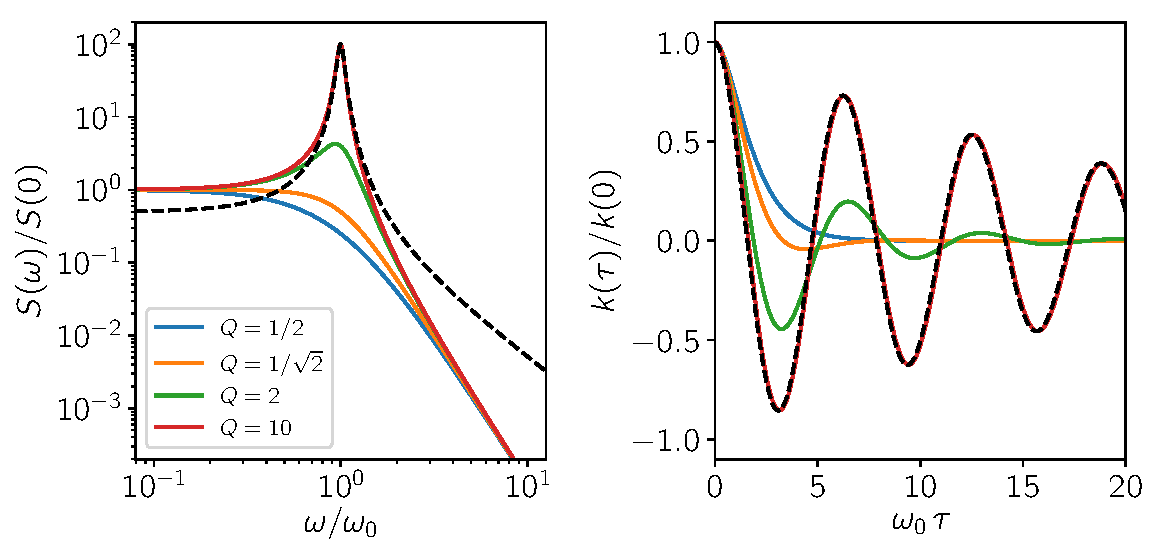
\includegraphics[width=0.9\textwidth]{figures/sho.pdf}
\caption{(left) The power spectrum of a stochastically-driven simple harmonic
    oscillator (\eqalt{sho-psd}) plotted for several values of the quality
    factor $Q$.
    For comparison, the dashed line shows the Lorentzian function from
    \eq{lorentz-psd} with $c_j = \omega_0/2\,Q = 1/20$ and normalized so that
    $S(d_j)/S(0) = 100$.
    (right) The corresponding autocorrelation functions with the same colors.
    \figurelabel{sho}}
\end{center}
\end{figure}


\section{Examples with simulated data}

\begin{enumerate}
\item an OU process
\item a full GenRP process
\item Some standard kernels: Matern, Exp-squared, etc.
\item A KISS-GP process
\end{enumerate}

\section{Examples with real data}

\subsection{Asteroseismic oscillations}

The asteroseismic oscillations of thousands of stars were measured using light
curves from the \kepler\ mission (\dfmtodo{cite}) and asteroseismology is a
key science driver for many of the upcoming large scale photometric surveys
(\dfmtodo{cite}).
Most asteroseismic analyses have been limited to relatively high
signal-to-noise oscillations because the standard methods based on statistics
of the empirical periodogram of the data cannot be used to formally propagate
the measurement uncertainties to the constraints on physical parameters
(\dfmtodo{CITE}) and more sophisticated methods are computationally expensive
and they scale poorly to the current state-of-the-art datasets (\dfmtodo{CITE
Brewer etc.}).

\genrp\ alleviates these problems by providing a physically motivated
probabilistic model that can be evaluated efficiently even for large datasets.
In practice, we will model the star as a mixture of stochastically driven
simple harmonic oscillators where the amplitudes and frequencies of the
oscillations are computed using a physical model and evaluate the probability
of the observed dataset using a Gaussian Process with a PSD given by a sum of
terms given by \eq{sho-psd}.
This gives us a method of computing the likelihood function for the parameters
of the physical model in $\mathcal{O}(N)$ operations and this can be combined
with standard non-linear optimization or posterior sampling methods to infer
constraints on the parameters for the given dataset.

To demonstrate this method, we will use a very simple heuristic model based on
\dfmtodo{CITE} where the model PSD is given by a mixture of 6 components with
amplitudes and frequencies specified by $\nu_\mathrm{max}$, $\Delta \nu$, and
several nuisance parameters.
The first term is used to capture the granulation ``background'' using
\eq{granulation-psd} with two free parameters $S_g$ and $\omega_g$.
The remaining 5 terms are given by \eq{sho-psd} where $Q$ is a nuisance
parameter shared between terms and the frequencies are given by
\begin{eqnarray}
\omega_{0,\,j} = 2\,\pi\,(\nu_\mathrm{max} + j\,\Delta\nu + \epsilon)
\end{eqnarray}
and the amplitudes are given by
\begin{eqnarray}
S_{0,\,j} =
    \frac{A}{Q^2}\,\exp\left(-\frac{[j\,\Delta\nu + \epsilon]^2}{2\,W^2}\right)
\end{eqnarray}
where $j$ is an integer running from $-3$ to 3 and $\epsilon$, $A$, and $W$
are shared nuisance parameters.
This model could be easily extended to include small frequency splitting and
$\nu_\mathrm{max}$ and $\Delta \nu$ could be replaced by physical parameters
like $\log g$.

\dfmtodo{Add plots etc.}

\begin{figure}[!htbp]
\begin{center}
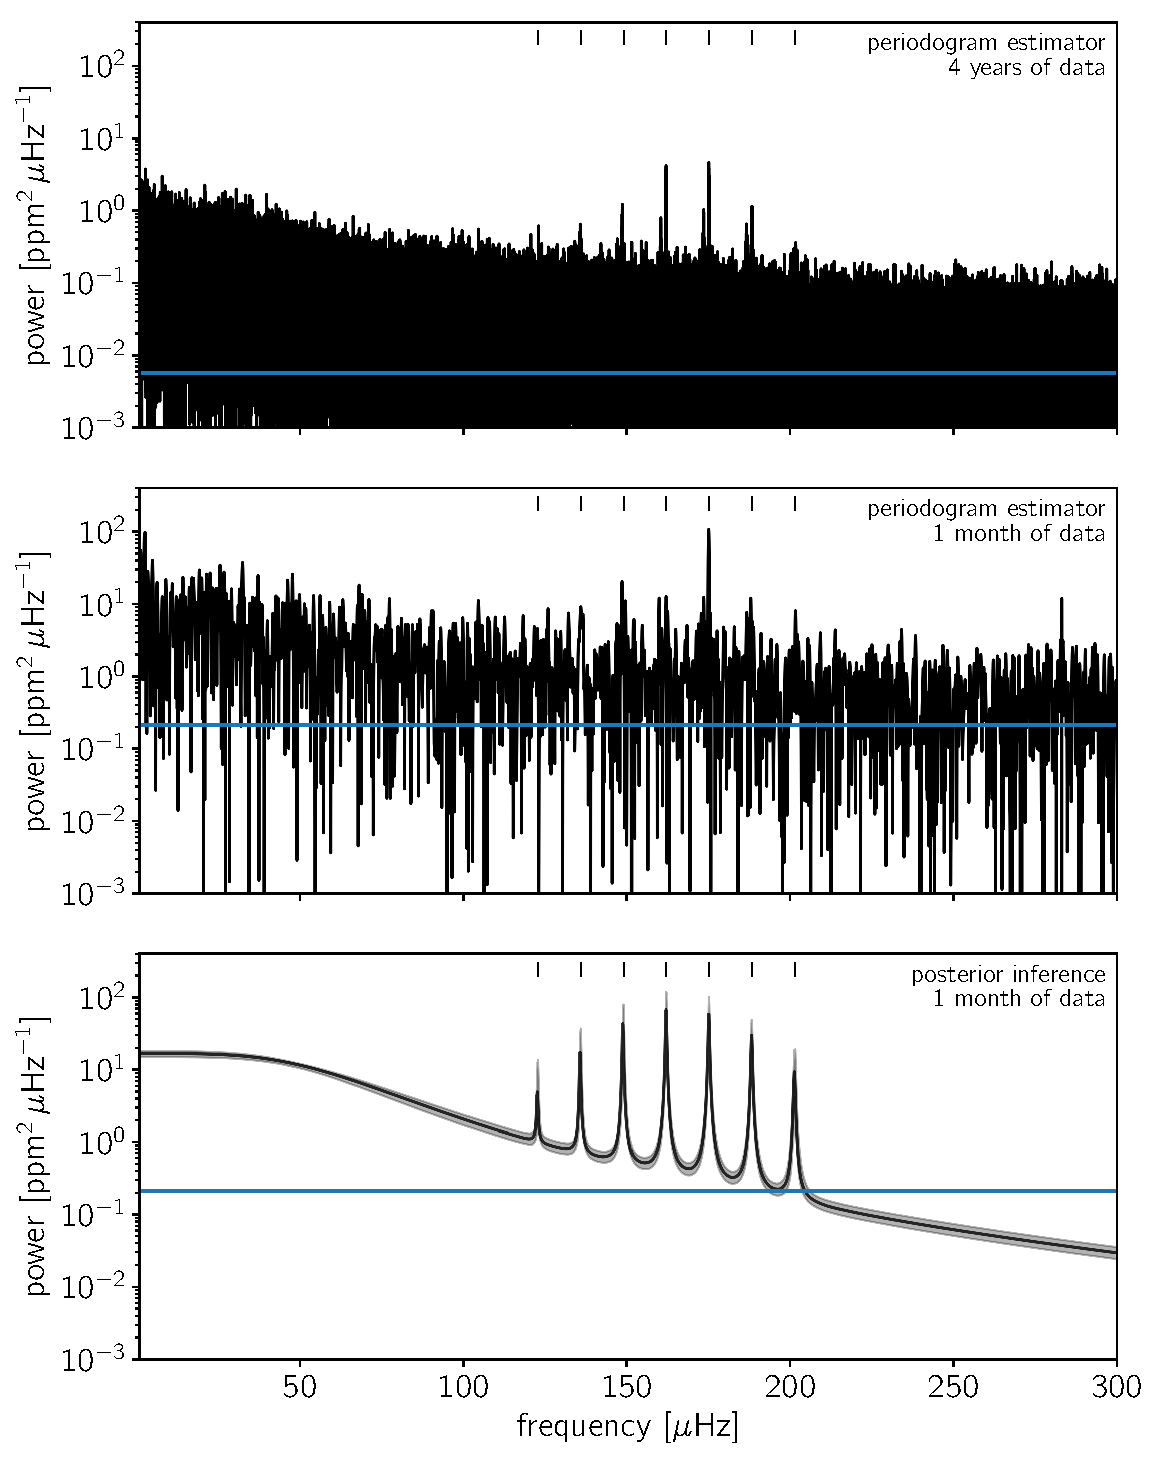
\includegraphics[width=0.9\textwidth]{figures/astero-11615890-comparisons.pdf}
\caption{A comparison between the empirical PSD and the posterior inference of
the PSD as a mixture of stochastically driven simple harmonic oscillators.
(top) The periodogram of the \kepler\ light curve for KIC~11615890 computed
    on the full four year baseline of the mission.
    The light gray curve shows the raw periodogram and the black curve has
    been smoothed with a Gaussian filter with \dfmtodo{SOME WIDTH}.
(middle) The same periodogram computed using about a month of data.
(bottom) The inferred power spectrum under the mixture of SHOs model described
    in the text.
    The black line shows the median of posterior PSD and the gray contours
    show the 68\% credible region.
    \figurelabel{astero}}
\end{center}
\end{figure}

\subsection{Stellar rotation}

For many stars it is possible

\begin{enumerate}
\item Asteroseismic target
\item Stellar rotation variability
\item Kepler with simulated transit
\item AGN
\end{enumerate}

\section{Comparisons to other methods}

Toeplitz, KISS-GP, CARMA, HODLR.

Limitations of GenRP: one-dimension, stationary, etc.


\section{Summary}



% DFM: I'm going to redistribute the following in other sections.

% Stars are variable, for better or worse:  their variability provides information about the properties
% of stars, but also results in noise that must be accounted for in detecting and characterizing their
% planetary systems.  When analyzing astronomical times series of stars, then, there are generally two
% goals:  1). to analyze the frequency spectrum and amplitude of stellar variability to better understand stellar
% properties and evolution, and/or 2). to account for correlated noise when modeling the stellar
% flux variability and spectral variations.

% A promising technique for addressing both of these goals is the Gaussian Process formalism
% \citep{Rasmussen2006,Gibson2012}.  The basis of this method is to assume that stellar variability
% is random, Gaussian noise, but that the random variability is correlated in time, and the nature of the
% correlations is completely specified by a correlation matrix.  In its simplest form, the
% correlation matrix is modeled with a time-independent autocorrelation function (although
% the time-independence can be relaxed), including a white-noise component that may vary
% with each exposure, and the autocorrelation function is described by a functional form that may be
% simply parameterized by a relatively small number of parameters, sometimes referred to as
% `hyper-parameters.'  The goal of spectral analysis is to measure the parameters which
% describe the autocorrelation function, thus inferring properties of the stellar variabilty
% which may be used to characterize properties of the star, such as the rotation period,
% the asteroseismic frequencies, or granulation noise known as `flicker' \citep{Aerts2010,Noyes1984,Bastien2013}.
% The goals of planet detection include measuring the Doppler shift of the star, measuring
% the decrement of flux as a planet transits a star, and/or measuring the times of transit to
% look for dynamical interactions between planets.  To properly account for the impact of
% stellar variability on the planet parameters requires treating correlations in the data, and
% to do so also requires evaluating the correlation matrix.

% The size of the correlation matrix, $N_{elements}$, scales as the square of the length of the time-series,
% $N_{element}=N_{time}^2$, so as time series grow in size, say $N_{time} =10^{5-6}$, the storage may become
% prohibitive, $N_{element} = 10^{10-12}$.  In addition, this matrix must be inverted and have
% its determinant evaluated to compute the likelihood function, which takes of order $N_{operations}
% = N_{time}^3 = 10^{15-18}$.  This becomes an impossible computational problem, which prohibits
% using long time series datsets, such as the {\it Kepler} dataset $N_{time} \approx 10^{5-6}$,
% {\it Spitzer} time series with $N_{time} \approx 10^5$, and Solar time series with
% $N_{time} \approx 10^7$.  So a faster means of solving for the likelihood is required in these
% cases.

% One promising solution is to use approximate techiques based upon the fact that correlation
% matrices display a great deal of symmetry.  This `hierarchical off-diagonal low-rank' (\texttt{HODLR})
% algorithm can make the storage and operations both scale in proportion to $N_{time}$, although the
% solver is only approximate \citep{Ambikasaran2013,Ambikasaran2016}.  In addition, the
% solver is complicated and can be challenging to use with general choices of kernel.  Another
% promising approximate technique is to use a uniform resampling of the dataset, and then
% rely on the structure of Toeplitz matrices, which require uniformly space time series,
% to obtain approximate solutions of the likelihood function \citep{WilsonNickisch2015},
% the `Kernel Interpolation for Scalable Structured Gaussian Processes' (\texttt{KISS-GP});
% this approach has the drawback of being approximate.  A third approach is to use a kernel
% based upon stochastic differential equations:  the `continuous auto-regressive moving-average'
% model \citep[aka \texttt{CARMA};][]{Kelly2014}.  This approach can model a stationary power-spectrum that
% is the combination of a number of Lorentzians, but has the disadvantage that the amplitudes
% of the Lorentzians are required to have a specific relation.  In addition, these
% techniques require a stationary kernel. {\color{red} Is this true for GEORGE?}

% The approach we explore in this paper is based upon a method developed by Press \&
% Rybicki twenty years ago \citep{Rybicki:1995}.  They observed that a correlation
% matrix consisting of a single exponential kernel has an inverse that is tri-diagonal.
% The coefficients and solution of a tri-diagonal matrix scale in proportion to $O(N_{time})$.
% They also indicated that a combination of two exponential kernels would have a simliar scaling,
% but they did not demonstrate how to extend this to more than two kernel components.

% A significant advance was made in generalizing the Press-Rybicki method to an
% arbitrary number of exponential kernels by utilizing the fact that the elements of
% such matrices can be written in terms of the products of components of two vectors,
% which are so-called semi-separable matrices \citep{Ambikasaran:2015}.  This `Generalized
% Rybicki-Press' (\texttt{GenRP}) approach
% has many advantages:  the computation time and storage both scale as $O(N_{time})$,
% the coefficients of the kernels need not be stationary, the computation of the
% likelihood is exact, and the algorithm is simple to implement, and thus is robust.
% Unlike the \texttt{CARMA} model, there is no restriction on the relation between
% the coefficients (except that the kernel needs to be positive definite).  Unlike
% \texttt{HODLR} and \texttt{KISS-GP},  the \texttt{GenRP} method is exact.  The main drawback
% of this approach is that the sum of exponential kernels with real coefficients can
% only represent a limited range of power spectra of auto-correlated time series:
% those which can be expressed the sum of Lorentzians that peak at zero frequency.

% However, this drawback turns out to not be significant:  the exponential kernel
% can also have a complex exponential coefficients (plus their complex-conjugates), and
% thus approximate an almost arbitrary autocorrelation function with enough terms, most
% importantly allowing for quasi-periodic kernels.  It turns out that the sum of Lorentzian
% components is a {\it very} good approximation of stellar variability spectra:  the
% activity and granulation noise due to stellar convection may be expressed in terms of zero-frequency
% Lorentzians \citep{1985ESASP.235..199H}, the asteroseismic oscillations may be expressed as non-zero frequency
% Lorentzians \citep{1990ApJ...364..699A,Gruberbauer2009}, and stellar rotation may be
% parameterized this way as well.  In this paper
% we extend the \texttt{GenRP} approach to kernels with complex exponentials, which when
% combined with the complex conjugate leads to damped harmonic auto-correlation functions
% which are flexible enough to describe a wide range of variability, and may still
% be solved in $O(N_{time}$ operations.

% We show that the extended matrix that embeds this multi-component kernel can be written
% in real notation, which speeds up the evaluation of the likelihood function,
% and allows optimization software to use automatic differential in computing
% derivatives of the likelihood function.

% The plan of the paper is...


% \section{Outline}
% \begin{enumerate}
%\item Non-parametric modeling of time series with correlated noise using Gaussian processes
%\item Assumptions:\\
%  a). Stationary noise (although this can be broken).\\
%  b). Gaussian
%\item Problem: can't handle large datasets - e.g. entire Kepler long-cadence; Spitzer light
%   curves; Solar curves; short-cadence.
%\item Solution(s):\\
%  a). HODLR \citep{Ambikasaran2013,Ambikasaran2016}\\
%  b). CARMA (Lorentzian power spectra, but with limitations) \citep{Kelly2014}\\
%  c). Tri-diagonal (Press \& Rybicki) \citep{Rybicki:1995}
%  d). KISS-GP \citep{WilsonNickisch2015} %Kernel Interpolation for Scalable Structured Gaussian Processes (KISS-GP) Andrew Wilson, Hannes Nickisch Proceedings of The 32nd International Conference on Machine Learning, pp. 1775-1784, 2015
%\item Problem: HODLR is tricky to use; CARMA requires certain relations between
%  coefficients of Lorentzians (right?); P\&R only works for up to 2 components + white noise
%\item Solution: Ambikasaran \citep{Ambikasaran:2015} shows how sum of exponential kernels can be solved in order
%   $O(N*p^2)$, where p is number of Lorentzians.
%  - Sum of Lorentzians is a good description of stellar variability:
%     - granulation has expoential (or sums of exponential) noise
%     - asteroseismic obeys sums of Lorentzians
%     - periodic variability due to spots/plages/etc. can also be
%       approximated by Lorentzian(s)
%\item Generalized Ambikasarn for complex coefficients (Hermitian).
% \item Performance:\\
%   a). Show $O(N*p^2)$ scaling\\
%   b). Show comparison to HODLR.\\
%   c). Show comparison to wavelet (ala Carter \& Winn).\\
%   d). Compare with CARMA Kallman filter(?).
% \item Various methods/formulae:\\
%   a). Likelihood computation.\\
%   b). Generating GP with particular covariance [yet to solve]. [ ]\\
%   c). Inferring particular components.\\
%   d). Computing derivatives of GPs (as used in RV methods).\\
%   e). Forecasting/interpolating.\\
%   f). Inferring confidence intervals.\\
%   g). Derivative of likelihood function with respect to kernel parameters.\\
%   h). Non-stationary GP (can the coefficients vary with time?).\\
%   i). Multi-band (each element of extended matrix becomes a matrix).
%   j). Approximating various kernels: Matern, exp(sin$^2$), Gaussian, etc.
% \item Generalization to non-stationary noise.
% \item Example application: TYC 3559\\
%   a). Entire long-cadence 17-quarter Kepler dataset (~65k data points).\\
%   b). Analysis of solar data.
%   c). CO2 Mauna Kea
%   d). TBD Computing derivatives of GPs (as used in RV methods).\\
%   e). TBD Forecasting/interpolating.\\
%   f). TBD Inferring confidence intervals.\\
%   g). Autodiff: Derivative of likelihood function with respect to kernel parameters.\\
%   h). TBD Non-stationary GP (can the coefficients vary with time?).\\
%   i). TBD Multi-band (each element of extended matrix becomes a matrix).

% \item Example application: TYC 3559\\
%   a). Entire long-cadence 17-quarter Kepler dataset (~65k data points).\\
%   b). Simulated datasets - hyperparameter/PSD inference.\\
%   c). Analysis of solar data?

% \item Possible future applications:\\
%   a). Inference of asteroseismic variability - ala Andrew Gordon Wilson \citep{2013arXiv1302.4245W}, but
%       with Lorentzians, not Gaussians.\\
%   b). Multi-waveband GPs.\\
%   c). RV interpolation.\\
%   d). Non-parametric phase functions.\\
%   e). Better calibration of the flicker log(g) relation.\\
%   f). Measurement of rotational periods - gyrochronology.\\
%   g). Doppler shifts in oscillating EBs.

% \item Appendix:
%   a). Description/summary of mathematics.\\
%   b). Description of code.
% \end{enumerate}

\section{Generalized Press-Rybicki}

The general problem to be solved for Gaussian Process analysis of stellar time series is to evaluate
the likelihood function,
\begin{equation}
{\cal{L}} = \ln{p(\mathbf{y}\vert {\mathbf{t},\bvec{\theta}},\bvec{\alpha})} = -\frac{1}{2}\ln{\vert \mathbf{K}(\bvec{\alpha}) \vert}
- \frac{N_{time}}{2} \ln{(2\pi)}
    - \frac{1}{2} {\mathbf r} (\bvec{\theta} ) ^T \mathbf{K}(\bvec{\alpha})^{-1} \mathbf{r}(\bvec{\theta}),
\end{equation}
where $\mathbf{y}$ are the measured time series (for example fluxes or radial velocities) at times
$\mathbf{t}$, while the data are modeled with a function $m(\mathbf{t};\bvec{\theta})$ (for example,
a transit model or Keplerian orbital model) which leaves residuals $\mathbf{r}(\bvec{\theta}) =
\mathbf{y} - m(\mathbf{t};\bvec{\theta})$. % Note: I'm using the same notation as the peerless project. -EA
The vector $\bvec{\alpha}$ specifies the parameters of the kernel, while the vector $\bvec{\theta}$
specifies the parameters of the physical model.  In addition to this likelihood, a prior may be placed on
the values of these model parameters (either the physical or kernel); the log of this prior may be
added to this log likelihood function.  Note that the kernel
parameters may also have a physical meaning, but they describe a noisy process, and thus affect
the correlated variability of stellar noise rather than a deterministic model as encapsulated in
$m(\mathbf{t};\bvec{\theta})$.

%The kernel is modeled as a sum of damped harmonics,
%\begin{equation}
%k_j(\tau) = a_0 \delta(\tau) + \sum_{j=1}^J a_j \exp{(-b_j \tau)} \cos{(-d_j \tau)} + b_j \exp{(-b_j \tau)} \sin{(-d_j \tau)},
%\end{equation}
%where $\tau > 0$ is a time-offset between data points, $c_j$ represents the decay
%in correlation with time and $d_j$ represents oscillations of period $P = 2\pi/d_j$, and
%$a_0 = \sigma^2$ is a white-noise component with $\delta(0) = 1$ and zero otherwise.  Formally
%the $\delta(\tau)$ function is a Kronecker delta function for which $\tau$ is the midpoint in
%time measured over a finite duration exposure time, and $\sigma$ is the standard deviation
%of the measured times if the correlated components are zero.

%Now, the damped harmonic kernel components may be rewritten as:
%\begin{equation}
% a_j e^{-\beta_R \tau} \cos{(\beta_I \tau)} = a_j \frac{1}{2}\left( e^{-(\beta_R + i \beta_I) \tau} +  e^{-(\beta_R + i \beta_I) \tau}\right),
%\end{equation}
%where $i^2 = -1$, which has the advantage of utilizing precisely the same form as the Rybicki-Press covariance
%matrix, and thus the Generalized Rybicki-Press algorithm may be applied as in \citet{Ambikasaran:2015}.
%The only difference is that the $\beta$ coefficients are now complex, $\beta = \beta_R + i \beta_I$,
%but otherwise the mathematical form of the extended matrix is identical, but with twice as many
%exponential kernel components as the real case.

Although the complex kernel is a straightforward extension to the \texttt{GenRP} formalism, there is a disadvantage
in computational speed:  complex arithmetic requires $\approx 3$ times as many operations as real
arithmetic.  In addition, it turns out that the complex conjugate component, $(c_j+id_j)^* = c_j - id_j$, in
the extended matrix gives a solution which, not surprisingly, is the complex conjugate of the
component $c_j + i d_j$;  thus the computation is redundant.  Finally, complex
arithmetic has the disadvantage that it is not included in automatic-differentiation packages,
which is what we would like to use to compute the derivative of the likelihood (as it is very difficult
to compute this explicitly!).

Consequently, we use the fact that $\exp{(id_j\tau)} =  \cos{(d_j\tau)} + i \sin{(d_j \tau)}$ to
rewrite the extended matrix in terms of real arithmetic using the fact that the imaginary number $i$
may be replaced by a $2\times 2$ anti-symmetric matrix,
\begin{equation}
\left(\begin{tabular}{ll}
0 & 1 \\
-1 & 0
\end{tabular}\right),
\end{equation}
while real numbers use the $2\times 2$ identity matrix, $\mathbf{I}$,
so that $\cos{(d_j\tau)} + i \sin{(d_j\tau)}$ may be rewritten as the rotation matrix
\begin{equation}
\left(\begin{tabular}{ll}
$\cos{(d_j\tau)}$ & $\sin{(d_j\tau)}$ \\
$-\sin{(d_j\tau)}$ & $\cos{(d_j \tau)}$
\end{tabular}\right).
\end{equation}
The algebraic properties of these matrices are identical to the complex numbers, but only involve
real components.
We accomplish this transformation in Appendix \ref{appendixa} by taking sums and differences of the complex
equations, resulting in a real extended matrix that is the same size as the complex matrix.
This transformation leads to about a factor of two in computational savings, but has the
additional advantage of allowing the automatic differentiation due to the use of real arithmetic.

\section{Kernel components}

%A stationary, smooth kernel may generally be expressed as a Taylor series for the $\tau \ne 0$ component,
%plus the white noise component:
%\begin{equation}
%k(\tau) = a_0 \delta(\tau) +  \sum_{j=0}^\infty c_j \tau^j.
%\end{equation}
%Note that this encompasses all smooth, time-stationary kernels, and generally $c_1 \le 0$ as
%correlated noise initially declines with separation in time.  We wish to approximate this
%as the sum of damped cosine kernels, and since this general kernel is symmetric in $\tau$, we
%can carry out the approximation in terms of sums of damped cosine kernel components
%\begin{equation}
%K_j(\tau,a_j,\beta_{R,j},\beta_{I,j}) = a_j \exp{(\beta_{R,j} \tau)}\cos{(\beta_{I,j} \tau)},
%\end{equation}
%which has a Taylor series expansion:
%\begin{eqnarray}
%\exp{(\beta_R \tau)}\cos{(\beta_I \tau)} &=& 1 - \beta_R \tau + \frac{1}{2}\left(\beta_R^2 - \beta_I^2\right)\tau^2 \\
%- \frac{1}{6} \left(\beta_R^3-3\beta_R\beta_I^2\right)\tau^3 &+& \frac{1}{24} \left(\beta_R^4+\beta_I^4-6\beta_R^2\beta_I^2\right) \tau^4+ O(\tau^5),
%\end{eqnarray}
%which may be continued to any order in $\tau$ as necessary.
%If an approximation to $k(\tau)$ is desired in a Taylor series to some high order $N$, this
%requires combining $N/2$ components of $K_j(\tau,a_j,\beta_{R,j},\beta_{I,j})$ with $\beta_{R,j}$ and $\beta_{I,j}$
%chosen to match the coefficients $c_j$.  Note that for $N=1$ we only require a damped exponential
%kernel with $\beta_I = 0$.
%
%Another way to view this is in the power spectrum of the gaussian process, which is the
%Fourier transform of the autocorrelation function.  The power spectrum of the $K_j$ kernel
%is a Lorentzian, for which the frequency is given by $\omega = \beta_{I,j}$, while the
%width of the Lorentzian is determined by $\beta_{R,j}$.  The functional form of this
%power spectrum is: {\color{red} Check that this is true.}
%\begin{equation}
%P(\vert f\vert) = a_j \beta_{R,j} \frac{1}{\beta_{R,j}^2 + (2\pi f - \beta_{I,j})^2},
%\end{equation}
%where $f$ is the frequency in Hz.  The counterpart to the Taylor series is the observation
%that a smooth distribution may be approximated arbitrarily precisely by summing together
%Lorentzians with various values of $(a_j,\beta_{R,j},\beta_{I,j})$.  In the case that
%a peak in the power spectrum is narrow at a specific frequency, then a small value of
%$\beta_{R,j}$ gives a narrow Lorentzian that may approximate that peak.  If the wings
%of the distribution decay faster than $f^{-2}$, then differences between Lorentzians
%can be arranged to cancel in the wings, giving features in the power spectrum that have
%narrower wings.

The functional form of $k_j$ may be used to approximate some commonly used Kernel components.
The squared exponential (Gaussian) kernel and the Mat\'ern kernels are commonly
used radial kernels, while the cosine kernel and the exponential-sine-squared kernels are
commonly used periodic kernels.  Linear combinations of our basis of damped cosine kernels may be
used to approximate each of these kernels to better than 1\% with various numbers of damped
cosine kernel components:
\begin{itemize}
\item {\bf Constant kernel.} A constant kernel component can be used to capture long-timescale
correlations in data, and can be represented exactly with $c_j= d_j =  0$.
\item {\bf Exponential kernel.} This kernel, $k(\tau) = e^{-\vert \tau/\tau_0\vert}$, is exactly
represented with $d_j=0$, $c_j= \tau_0^{-1}$.
\item {\bf Cosine kernel.} The cosine kernel, $k(t) = \cos{\left(\frac{2\pi}{P} \vert \tau \vert\right)}$,
may be represented exactly with $c_j=0$ and $d_j= \frac{2\pi}{P}$.
\item {\bf Squared exponential.} The squared exponential or Gaussian kernel, $G(z)=e^{-z^2/2}$,
has the behavior of declining steeply at large time separation, is an even function, and has $c_1$ = 0.
Likewise, the Fourier transform of the squared exponential kernel is $\hat G(\omega) = e^{-\omega^2/2}$,
which also declines steeply at large $\omega$;  this doesn't match the more gradual decline of the
power spectrum of a damped sinuosoid.  Nevertheless, the squared exponential kernel may be well approximated
by the sum of four exponential kernels:
\begin{eqnarray}
G(z) &\approx& 63.119512 e^{-1.479579 z} -32.173615 e^{-1.593691 z} -29.425156 e^{-1.388929 z}\\
&+& e^{-1.383928 z} \left[-0.519196\cos{(1.883396 z)} +0.285478 \sin{(1.883396 z)}\right] \\
\end{eqnarray}
which has an accuracy of better than $<3\times 10^{-3}$ for all z, and the power spectrum has
been constrained to be positive.
\item {\bf Mat\'ern $p+1/2$ kernel.}  The Mat\'ern kernel is given by:
\begin{equation}
C_{p+1/2}(x) = \sigma^2 e^{-\sqrt{(2p+1)}x} \frac{\Gamma(p+1)}{\Gamma(2p+1)}
\sum_{i=0}^p \frac{(p+i)!}{i!(p-i)!} (\sqrt{(8p+4)}x)^{p-i},
\end{equation}
where $p$ is a positive integer.  In the limit $p\rightarrow \infty$, this becomes the
squared exponential kernel: $C_\infty(x) = \sigma^2 e^{-x^2/2}$.  But, for small
values of $p$, the Mat\'ern kernel may be approximated well by the sum of
$2p$ exponential kernels.  The exponential kernel is the Mat\'ern 1/2 kernel,
$C_{1/2}(x) = \sigma^2 e^{-x}$ ($p=0$), while
$p=1$ is relevant to stellar variability, which we describe next.
\item {\bf Mat\'ern 3/2 kernel.}  The Mat\'ern $3/2$ ($p=1$) kernel is given by:
\begin{equation}
k_{3/2}(\tau) = C_{3/2}(\tau/\tau_0) = (1+v)e^{-v},
\end{equation}
where $v = \sqrt{3}\vert \tau/\tau_0\vert$.  This kernel has a Fourier transform\footnote{Using the normalization convention:
$\hat f(\omega) = \frac{1}{\sqrt{2\pi}} \int_{-\infty}^\infty f(t) e^{i\omega t} dt$}  of
\begin{equation}
\hat k_{3/2}(\omega) = \frac{\tau_0 6^{3/2}}{\pi^{1/2}} (3+\tau_0^2\omega^2)^{-2},
\end{equation}
where $\omega = 2\pi f$.  This kernel may be well approximated by the sum of two exponential kernels:
\begin{equation}
k_{3/2}(\tau) \approx (1-b)e^{-v}+be^{-v\frac{b-1}{b}},
\end{equation}
where $b \gg 1$ is a dimensionless parameter; this approximation is exact in the limit $b \rightarrow \infty$.  For
large values of $b$, the maximum error of the approximation scales as $2/(e^2b) \approx 0.27/b$; for
$b=100$, the error in this approximation is $<0.3$\%.  Note that the two exponential terms
have opposite signs, which may lead to numerical instability for values of $b$ that
are large.

One advantage of the Mat\'ern 3/2 kernel is that it is smooth across
$\tau=0$ since its derivative is zero at $\tau=0$.  The exponential kernel {\it does not}
have this property, which leads to qualitatively different noise properties on small
timescales due to the sharpness of the exponential kernel at $\tau=0$.  The Mat\'ern 3/2 kernel
turns out to be similar to the observed properties of stellar activity and granulation, and thus the approximate
formula is simultaneously physically relevant and computationally convenient.
The power spectrum of a single exponential scales as $f^{-2}$ at high frequency,
while the Mat\'ern kernel scales as $f^{-4}$ which more closely matches the power
spectrum due to activity and granulation in the Sun \citep{2004A&A...414.1139A,Michel:2009}.
\item {\bf Mat\'ern 5/2 kernel.}  The Mat\'ern 5/2 kernel is given by
\begin{equation}
k_{5/2}(t) = C_{5/2}(y) = \sigma^2 (1+y+y^2/3)e^{-y},
\end{equation}
where $y = \sqrt{5}\vert \tau/\tau_0\vert$.  The Fourier transform is:
\begin{equation}
\hat k_{5/2}(\omega) = \frac{2\tau_0 10^{5/2}}{3\pi^{1/2}} (5+\tau_0^2\omega^2)^{-3}.
\end{equation}
This kernel may be approximated well by the sum of four exponential kernels
\begin{eqnarray}
k_{5/2}(\tau) &\approx& -147.6965573 e^{-1.0097610 y} + 85.8875034 e^{-1.0621734 y}\\
 &-&4.6540017 e^{-0.8353745 y} + 67.4630744 e^{-0.9160394 y},
\end{eqnarray}
which is accurate to $<4\times 10^{-6}$ for $y \le 10$.
The Fourier transform has a steeper dependence at large frequencies, $f^{-6}$, and as we are not aware of a stellar
power spectrum that requires a steeper spectrum than this, we forego approximating further Mat\'ern kernels.
\item {\bf Exponential-sine-square kernel.}  This kernel is a periodic, positive valued kernel
which has been used to model quasi-periodic stellar variability due to star spots.   It is
given by $E(w,\Gamma) = e^{-\Gamma \sin^2{w}}$ where $w = \frac{\pi}{P}\vert \tau \vert$, which may be
expanded as a series in $\cos{(2kw)} = \cos{\frac{2\pi}{P} k \vert \tau \vert)}$,
with $k \in \mathbb{N}$.  We have expanded this to $k=4$, and fit for the coefficients, giving:
\begin{equation}
E(w,\Gamma) \approx \sum_{k=0}^4 \left(c_{k,1}+c_{k,2} e^{-c_{k,4}\Gamma^{c_{k,3}}}\right) \cos{(2kw)},
\end{equation}
with $c_{0,1}=0.24999, c_{0,2}=0.752803, c_{0,3}=0.960477, c_{0,4}=0.643393$ for $k=0$,
$c_{1,1}=0.450851, c_{1,2}=-0.445338, c_{1,3}=0.960477, c_{1,4}= 1.18102$ for $k=1$,
$c_{2,1}=0.206593, c_{2,2}=-0.207361, c_{2,3}=1.65902, c_{2,4}= 0.210641$ for $k=2$,
$c_{3,1}=0.0728449, c_{3,2}=-0.0729381, c_{3,3}=2.43149, c_{3,4}= 0.0471224$ for $k=3$, and
$c_{4,1}=0.019204, c_{4,2}=-0.0192129, c_{4,3}=3.27977, c_{4,4}= 0.0114198$ for $k=4$.
This approximation is accurate to better than 0.6\% for $\Gamma < 3$, with a standard
deviation of 0.1\%.
\end{itemize}

Examples of the foregoing kernels and their approximations are shown in Figure \ref{kernel_approx}.
It is clear from this figure that these standard kernels are well approximated by the sums
of between two and five damped cosine kernels, demonstrating that these form an adequate set
for modeling a wide range of kernel behaviors.

\begin{figure}[!htbp]
\begin{center}
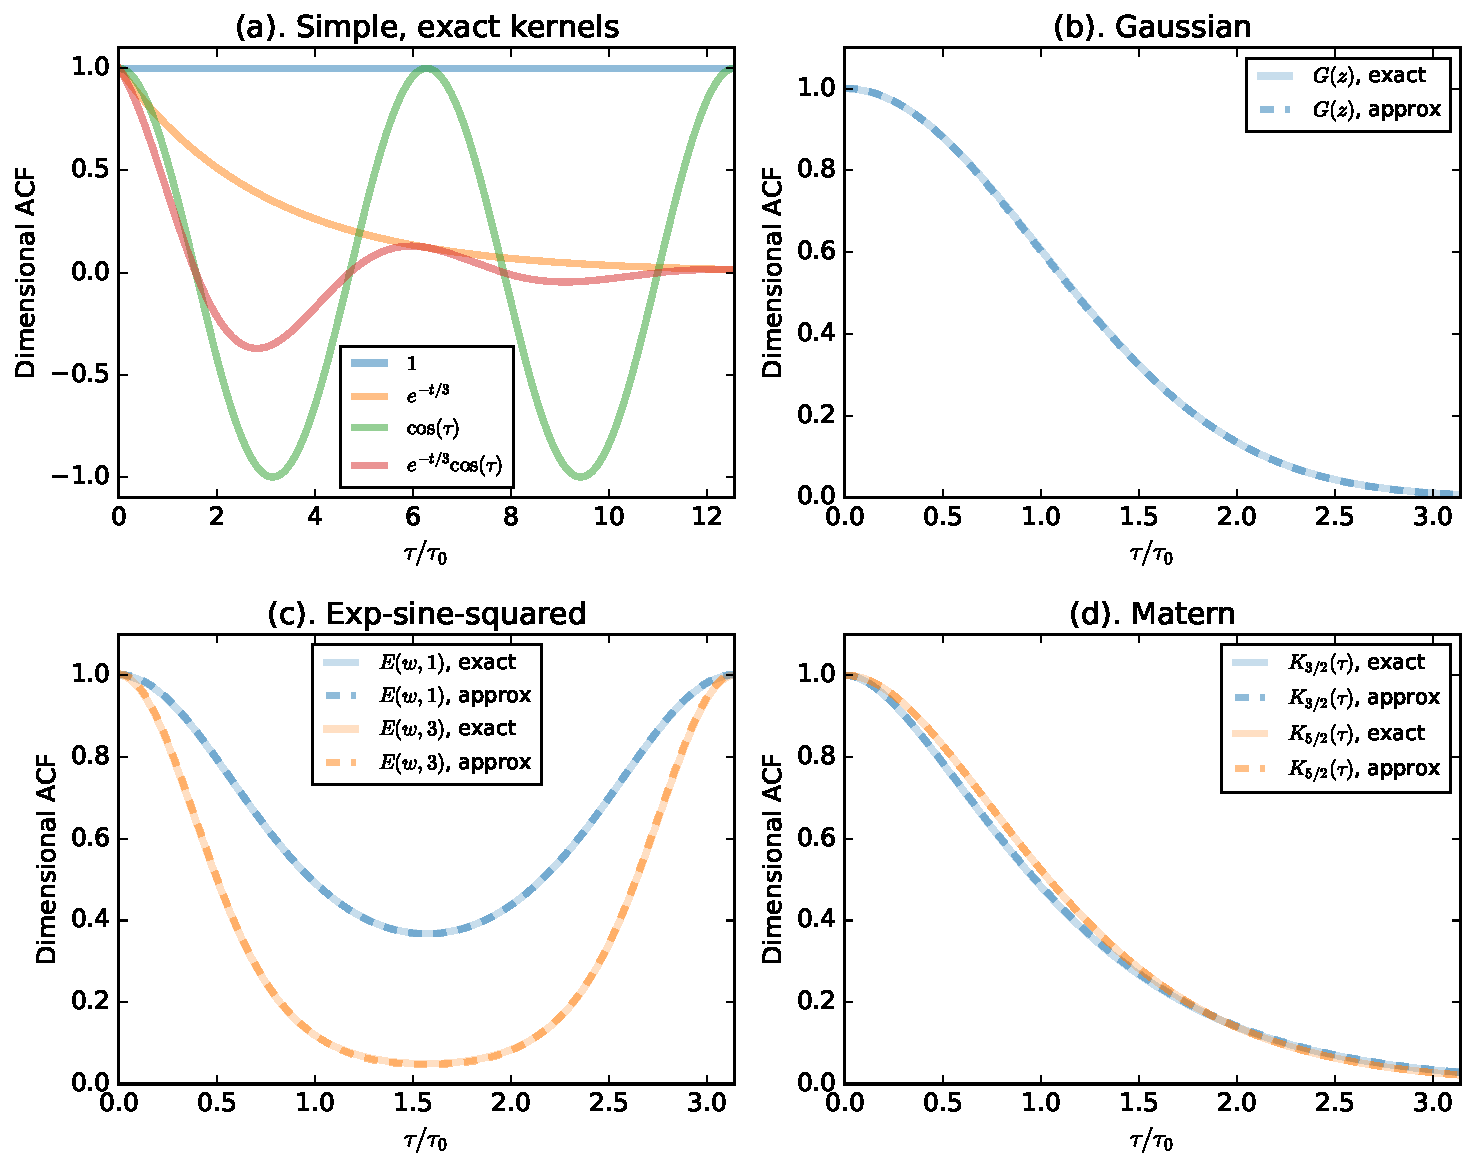
\includegraphics[width=\textwidth]{./approximate_kernels/kernel_approx.pdf}
\caption{Approximation of various kernels with the sums of damped cosines.
(a). Kernels that may be expressed exactly: constant (dark grey), exponential (cyan),
cosine (olive), and damped cosine (salmon).
(b). Approximation of the squared-exponential (Gaussian) kernel (pink) with three
damped cosine kernels (magenta). (c). The approximation of the exponential-sine-squared
kernel with $\Gamma =1$ (blue) and $\Gamma = 3$ (green). (d). Two Mat\'ern kernels,
$k_{3/2}$ (yellow/brown) and $k_{5/2}$ (violet).  The Mat\'ern 3/2 kernel
is approximated with $b=100$. The exact kernels are solid, while approximate are dashed.}
\label{kernel_approx}
\end{center}
\end{figure}

A standard practice in constructing kernels for solving problems with Gaussian processes
is to add or multiply the preceding standard kernel components.  In the case of damped cosine
kernels, the product of two kernels is:
\begin{eqnarray}
k_j(\tau)k_k(\tau) &=&
\frac{1}{2} e^{-(c_j+c_k) \tau} \left((a_ja_k+b_jb_k)\cos{\left[(d_j-d_k)\tau\right]} + (a_jb_k-a_kb_j)\sin{\left[(d_j-d_k)\tau\right]} \right. \\
 &+&\left.(a_ja_k-b_jb_k)\cos{\left[(d_j+d_k)\tau\right]} -(a_jb_k-a_kb_j)\sin{\left[(d_j+d_k)\tau\right]}\right),
\end{eqnarray}
which is the sum of two damped sinusoidal kernels.  Thus, only addition is necessary to
construct new kernels from the product of damped sinuosidal kernels.

The upshot is that the damped sinusoid is an expressive basis kernel that may be used
to represent a wide range of autocorrelation functions relevant for stellar variability, and
more.
We recommend using a series of sums of damped sinusoids (in which some parameters may be
fixed to specified values to represent particular kernels) to model different amplitudes
and timescales of variability.  If an initial estimate of the power spectrum or
autocorrelation function is available, then these may be fit with this series to
initialize the coefficients of the damped sinusoid kernel components.
Since a Gaussian Process
must be positive definite, we recommend modeling the logarithm of $a_j$, $b_j$,
$c_j$, and $d_j$ to enforce this to be the case.  One caveat is
that to produce certain kernels, a negative value of $a_j$ or $b_j$ is needed (such
as the Mat\'ern 3/2 kernel).  In this case, the value of the sum of
two coefficients may be sampled from a logarithm, while the individual
values are allowed to be negative;  this will enforce the positive definite
constraint, but may allow for other constraints, such as an autocorrelation
function which has a derivative of zero at $\tau = 0$.

%\subsection{Derivative of likelihood with respect to Kernel parameters}
%
%The derivative of the likelihood can be computed in $O(N)$ operations as follows.
%
%The derivative of the log likelihood with respect to model parameters ${\bf x}$ is given by:
%\begin{equation}
%    \frac{\partial \ln{\cal L}}{\partial x_i} = (\ln{\cal L})^\prime = -\frac{1}{2}\sum_i \frac{K_{ii}^\prime}{K_{ii}}
%    - \frac{1}{2} {\bf y}^T {\bf K}^{-1} {\bf K}^\prime {\bf K}^{-1} {\bf y},
%\end{equation}
%where $^\prime$ means the derivative wrt $x_i$.
%The kernel may be written as:
%\begin{equation}
%    K_{ij}({\bf \alpha},{\bf \beta}) = \left\{
%    \begin{array}{cc}
%       w_i + \sum_{l=1}^J \alpha_l & j = i \\
%       \sum_{l=1}^J \alpha_l \exp{(-\beta_l |t_i-t_j|)}  & j \ne i
%    \end{array}
%    \right.
%\end{equation}
%Since this equation is the sum of $J$ semi-separable matrices, then applying the product rule to compute the derivative will give a single semi-separable matrix for the derivative with respect to each kernel parameter.
%
%Now, letting ${\bf x} = (w,{\bf \alpha},{\bf \beta})$, then the derivative may be written as:
%\begin{eqnarray}
%    \frac{\partial K_{ii}}{\partial w} &=& \delta_{ij}\\
%    \frac{\partial K_{ij}}{\partial \alpha_k} &=&
%     \left\{
%    \begin{array}{cc}
%       1 & j = i \\
%        \exp{(-\beta_k |t_i-t_j|)}  & j \ne i
%    \end{array}
%    \right.\\
%    \frac{\partial K_{ij}}{\partial \beta_k} &=&
%     \left\{
%    \begin{array}{cc}
%       0  & j = i \\
%        -\alpha_k|t_i-t_j|\exp{(-\beta_k |t_i-t_j|)}  & j \ne i
%    \end{array}
%    \right.
%\end{eqnarray}
%The first term in the derivative of the likelihood can be computed in $O(N)$
%evaluations, while the second term can be computed in three steps:
%\begin{itemize}
%\item First, solve ${\bf z_1} = {\bf K}^{-1}{\bf y}$ with the GRP solver.
%\item Next, create an e
%\end{itemize}
%Writing this term out:

\section{Summary}

Although we have in mind application of this fast method to stellar variability,
the method is general for one-dimensional GP problems, and may be applied to
other problems.    Within astrophysics, correlated noise (due to the environment,
detector, or modeling uncertainty) may be present in
gravitational wave time series, and so Gaussian processes may be a way to address
this problem \citep{Moore2016}.  Accreting black holes show time series which
may be modeled by correlated noise \citep{Kelly2014};  indeed, this was the
motivation for the original technique developed by Rybicki \& Press \citep{1992ApJ...398..169R,Rybicki:1995}.
This approach may be broadly used for characterizing quasar variability \citep{2010ApJ...721.1014M},
measuring time lags with reverberation mapping \citep{2011ApJ...735...80Z},
and modeling time delays in multiply-imaged gravitationally-lensed systems \citep{1998ApJ...507..108P}.

Outside of astronomy, this technique may have application to seismology \citep{Robinson1967},


\vspace{1.5em}
All of the code used in this project is available from
\url{https://github.com/dfm/GenRP} under the MIT open-source software
license.
This code (plus some dependencies) can be run to re-generate all of the
figures and results in this paper; this version of the paper was generated
with git commit \texttt{\githash} (\gitdate).

\section{Solving for log likelihood with extended matrix}

Here we summarize \citet{Ambikasaran:2015}, and then point to appendix
for how to do this with oscillating kernels.

\section{Training}

May use derivative of likelihood + BFGS-B to optimize kernel parameters.

Q: How do we determine how many kernels to use?

\section{Discussion}

There are three primary applications we envision for the \genrp\ formalism: 1).\ modeling
the variability of an astrophysical system to infer it properties; 2).\
accounting for astrophysical variability as a source of noise when trying to detect
additional phenomena; 3).\ interpolating or extrapolating variability to future or missing
times.  Some examples of the first are determining the characteristic
variability timescale of a quasar, measuring the asteroseismic variation of a star,
or detection of quasi-periodic variability in a high-energy source.  Examples of the
second are detecting transiting exoplanets and correcting for stellar activity in
radial velocity measurements. Examples of the third are measuring time delays in
multiply-imaged gravitationally lensed sources and reverberation mapping of AGN.

\subsection{Application to stellar variability, transiting exoplanets}

Our background is in studying transiting exoplanets, a field which has only recently begun
to adopt full covariance matrices in analyzing the noise in transiting planet lightcurves.
One promising early attempt at accounting for correlated noise was the wavelet approach
of Carter \& Winn (2010).  Their technique allowed for a power-law spectrum for the
noise scaling as $\omega^{-\alpha}$, which unfortunately is not a normalizable, nor
physically-accurate, description of stellar variability.  Their approach runs in
${\cal O}(N)$ time for $\alpha=1$, which is `flicker' or pink noise;  however, this
particular type of noise overpredicts the power spectrum at low frequency compared
to the granulation power spectrum.  It also cannot describe quasi-periodic noise.

Further progress was made by parameterizing the covariance matrix with simple,
analytic functions that describe the autocorrelation function.  The parameters
of these functions can then be optimized to best match the observed variability
pattern of the residuals (after subtracting a transit model).  The disadvantage of
this approach is that the functions used are chosen somewhat arbitrarily (e.g.\
the exponential-squared function), and the Cholesky decomposition of the covariance
matrix for computing the likelihood takes ${\cal O}(N^3)$ operations which prohibits
application of this technique to large datasets.

Given the drawbacks of these approaches, the \genrp\ formalism allows both a fast
computation of the likelihood in ${\cal O}(N)$ time, as well as a functional form
that accurately describes stellar variability due to the relation to the simple
harmonic oscillator power spectrum, which is an analog of stellar asteroseismic
oscillations.  As higher signal-to-noise observations of transiting exoplanet systems
are obtained, the effects of stellar variability will more dramatically impact the
correct inference of planetary transit parameters, and so we expect that \genrp\
will be important for transit timing, transit spectroscopy, Doppler beaming,
phase functions, and more.

%\section{Prediction/interpolation}
%
%Precition/interpolation involves constructing a matrix of covariances
%between the (noisy) training set and the times at which we wish to
%predict or interpolate data points.   If our training times are given by
%${\bf t}$, while the predicted times are given by ${\bf t}_*$, then
%mean values at the predicted times are given by (RW 2.23):
%\begin{eqnarray}
%\bar f_{*,k} &=& \sum_j k(t_{*,k},t_j) b_j,\\
%&=& \sum_j \sum_p \alpha_p e^{-\beta_p \vert t_{*,k}-t_j\vert} b_j,\\
%&=& \sum_p \alpha_p \sum_j e^{-\beta_p \vert t_{*,k}-t_j\vert} b_j,\\
%y_k &=& \sum_j k(t_j,t_k) h_j,
%\end{eqnarray}
%where the latter equation may be solved for ${\bf h}$ using the extended
%matrix formalism.  Let the length of ${\bf t}_*$ be $M$; then, the
%matrix $k({\bf t}_*,{\bf t})$ has a size $M \times N$, and so a total
%of $MN$ multiplications is required to obtain the predicted values.
%If $M$ is large, this can become quickly prohibitive.  It turns out
%that the structure of the sum of exponential kernels may be exploited
%to obtain the predicted mean in of order $J(M+N)+J^2N$ multiplications,
%i.e.\ a linear scaling with the total number of data points, which can
%be much fewer if $M$ is large.
%
%The procedure works as follows:
%\begin{itemize}
%\item Sort ${\bf t}$ and ${\bf t}_*$ in time order.
%\item Starting with the smallest value of ${\bf t}_*$, $t_{*,1}$,
%compute:
%\begin{eqnarray} \label{prediction}
%\bar f_{*,k} &=& \sum_p \alpha_p \left[\epsilon^+_{p,k} + \epsilon^-_{p,k}\right]\\
%\epsilon^+_{p,k} &=& \sum_{j \forall t_{*,k} > t_j} e^{-\beta_p (t_{*,k}-t_j)} h_j\\
%\epsilon^-_{p,k} &=& \sum_{j \forall t_{*,k} \le t_j} e^{-\beta_p (t_j-t_{*,k})} h_j,
%\end{eqnarray}
%where we have separated out the training times before and after the predicted time $t_{*,k}$.
%
%\item Next, we update the coefficients recursively:
%\begin{eqnarray}
%\epsilon^+_{p,k} &=& e^{-\beta_p (t_{*,k}-t_{*,k-1})} \left[\epsilon^+_{p,k-1} + \sum_{j \forall t_{*,k} > t_j \ge t_{*,k-1}} e^{-\beta_p (t_{*,k}-t_j)} h_j\right]\\
%\epsilon^-_{p,k} &=& e^{-\beta_p (t_{*,k}-t_{*,k-1})} \left[\epsilon^-_{p,k-1} - \sum_{j \forall t_{*,k} > t_j \ge t_{*,k-1}} e^{-\beta_p (t_j-t_{*,k})} h_j\right].
%\end{eqnarray}
%With these updates, we can then use equation \ref{prediction} to compute the expected
%mean at $t_{*,k}$ with an additional $J$ operations.  Since there are $N$ values of
%$t_k$, the number of operations needed to update $\epsilon$ is of order $J(N+M)$, and
%so this procedure avoids a heavy computational burden.
%
%The variance may be handled in a similar manner, but with $J^2$ coefficients
%to recursively update. For example, if $t_{*,k} > t_j \forall j,k$ then:
%\begin{eqnarray}
%cov(f_{*,k}) &=&  k(t_{*,k},t_{*,k}) - \sum_p \sum_q \alpha_p \alpha_q e^{-\beta_p(t_{*,k}-{\bf t}^T)} k({\bf t},{\bf t})^{-1} e^{-\beta_q (t_{*,k}-{\bf t})},\\
%&=& k(0) - \sum_p \sum_q \alpha_p \alpha_q \zeta_{p,q,k},\\
%\zeta_{p,q,k} &=&   e^{-\beta_p(t_{*,k}-{\bf t}^T)} k({\bf t},{\bf t})^{-1} e^{-\beta_q (t_{*,k}-{\bf t})},\\
%&=&  e^{-(\beta_p+\beta_q)(t_{*,k}-t_{*,k-1})} \zeta_{p,q,k-1}.
%\end{eqnarray}
%The recursive updates to the $\zeta_{p,q,k}$ parameters can be made at each step.
%\end{itemize}
%
%Problem:  if we have the case that the datapoints are interspersed, and if the sign changes,
%then we need to resolve $K^{-1} e^{-\beta_q \vert t_{*,k}-{\bf t}\vert}$.  However, maybe we can
%just solve for the difference in fewer operations? {\bf TBD}

\acknowledgments
It is a pleasure to thank
Sivaram Ambikasaran,
Ruth Angus,
Will Farr,
and
David W.\ Hogg
for helpful contributions to the ideas and code presented here.

EA acknowledges support from NASA grants NNX13AF20G, NNX13AF62G, and
NASA Astrobiology Institute's Virtual Planetary Laboratory, supported
by NASA under cooperative agreement NNH05ZDA001C.

This research made use of the NASA \project{Astrophysics Data System} and the
NASA Exoplanet Archive.
The Exoplanet Archive is operated by the California Institute of Technology,
under contract with NASA under the Exoplanet Exploration Program.

This paper includes data collected by the \kepler\ mission. Funding for the
\kepler\ mission is provided by the NASA Science Mission directorate.
We are grateful to the entire \kepler\ team, past and present.

These data were obtained from the Mikulski Archive for Space Telescopes
(MAST).
STScI is operated by the Association of Universities for Research in
Astronomy, Inc., under NASA contract NAS5-26555.
Support for MAST is provided by the NASA Office of Space Science via grant
NNX13AC07G and by other grants and contracts.

\facility{Kepler}
\software{%
    % \project{ceres} \citep{Agarwal:2016},
    % \project{corner.py} \citep{Foreman-Mackey:2016},
    % \project{emcee} \citep{Foreman-Mackey:2013},
    % \project{george} \citep{Ambikasaran2016},
	% \project{matplotlib} \citep{Hunter:2007},
	% \project{numpy} \citep{Van-Der-Walt:2011},
	% \project{scipy} \citep{Jones:2001}.
}

\appendix

\section{Implementation details}\sectlabel{implementation}

Here we adapt the generalized Rybicki-Press (GRP) algorithm to handle periodic kernels.  We
follow closely the notation and equations given in \citet{Ambikasaran:2015}.  We start
with the observation that a damped sinusoid correlation function may be decomposed into the sum of two
exponential functions:
\begin{eqnarray}
k_j(\tau) &=& a_j e^{-c_j\tau} \cos{(-d_j\tau)} + b_j e^{-c_j\tau} \sin{(-d_j \tau)}\\
 &=& \frac{1}{2}(a_j+ib_j)\left[e^{-(c_j+id_j) \tau}+e^{-(c_j-id_j) \tau}\right],
\end{eqnarray}
where $c_j + id_j$ is the complex kernel parameter and $d_j = 2\pi/P$
is the frequency of oscillation of the kernel with period $P$.

Now, the damped sinusoid kernal may be included in the GRP algorithm
using the above two exponential kernels.  This
requires the algorithm to use complex arithmetic, which has several disadvantages:
1).\ complex arithmetic is more expensive by a factor of 2-3; 2).\ the complex conjugate equation
is redundant as it turns out that $l_2 = l_1^*$, $r_2 = r_1^*$, and $x_i = x_i^*$ (i.e.\ $x_i$ is
real), meaning that the same equations are being solved twice for the real and complex components;
and 3).\ if the derivative of the likelihood is computed with automatic
differentiation (AD), most AD algorithms require real variables.

Given these drawbacks, we instead modify the GRP algorithm to use a combination of two real
components rather than two complex components;  this addresses all three of these drawbacks
simultaneously.  The one cost is that the banded extended matrix has a bandwidth which is
larger by one, both above and below the diagonal.

Rather than using $c_j+id_j$ and its complex conjugate as components of the kernel, we instead
find the real and imaginary components of the complex equation by taking the
sum and difference of the $c_j+id_j$ and $c_j-id_j$ equations (divided by 2 and $2i$, respectively),
and then discard the $c_j-id_j$ equation, which is redundant.  This keeps the same number of
additional equations for each $(c_j,d_j)$ with non-zero imaginary component (four additional
equations in the extended matrix), but converts the complex equations to real, thus avoiding
complex arithmetic, while the kernel components with $d_j=0$ still only have two
additional components in the extended matrix.  The extended matrix adds an extra band above
and below the diagonal when the $c_j+id_j$ and $c_j-id_j$ equations are combined since this
mixes the components of the original equations which are shifted by one column from one
another.  We will enumerate the number of $d_j=0$ cases as $J_0$, while the total number
of $c_j$'s is still $J$.  This gives a total number of equations to be solved with the
extended matrix of $N_{ex}= (4(J-J_0)+2J_0+1)\times(N-1)+1$, where $N$ is the number of data
points.

% Reprint Ambikasaran equations (59)-(61)

For the complex values with $d_j \ne 0$, the equations are modified as follows.  We introduce complex
auxiliary vectors $l_n = g_n - i h_n$, with $n \in \{1,2,...,N\}$ and $l_1 = 0$; $r_n =
u_n - i v_n$, with $n \in \{2,...,N\}$ and $r_{N+1} = 0$.  Note that we have defined the
imaginary component as being negative for aesthetic reasons:  this yields a symmetric extended
matrix (unfortunately the extended matrix has negative eigenvalues, making it non positive-definite,
so that Cholesky decomposition cannot be applied; nevertheless we prefer to use a symmetric
set of equations, and since the values of these variables are discarded in the end, their sign
is irrelevant).  The length of the vectors $l_n$ and $r_n$
is the number of kernel components, $J$;  we denote the individual elements of these vectors
as $g_{n,j}+ih_{n,j}$ and $u_{n,j}+iv_{n,j}$, $j \in \{1,...,J\}$.  Note that the first $J_0$ elements we take
to be the kernels with $d_j=0$, and for these we do not include the imaginary component
equations, which are unnecessary and only add extra computation time.  We also define vectors $\phi$ and $\psi$ with
complex components as well:  $\gamma_n = \phi_n + i\psi_n = \left[\exp{(-(c_1+id_1) t_{n,n+1})} ... \exp{(-(c_J+id_J) t_{n,n+1})}\right]^T
$.  The individual elements are given by $\phi_{n,j} = e^{-c_j t_{n,n+1}}
\cos{(d_j t_{n,n+1})}$ and $\psi_{n,j} = -e^{-c_j t_{n,n+1}}\sin{(d_j t_{n,n+1})}$.
Equation (61) becomes:
\begin{equation} \label{Amb61}
% See 9/2/2016 notes
% Use n rather than k for {1...N} - use g, h & u, v?
% \gamma & \phi - real & imaginary
\sum_{j=1}^J \left(\frac{a_j}{2} g_{n,j} +\frac{b_j}{2} h_{n,j}\right)+ \frac{d}{2} x_n + \sum_{j=1}^J \left[
\phi_{n,j} u_{n+1,j} + \psi_{n,j} v_{n+1,j}\right] = \frac{y_n}{2},
\end{equation}
for $j \in \{1,...,J\}$ and $n \in \{1,...,N\}$, where $y_j$ is the $j$th data point.  There is no imaginary component to equation (61)
in \citet{Ambikasaran:2015}.

Equation (60) in \citet{Ambikasaran:2015} has real and imaginary components:
\begin{eqnarray} \label{Amb60}
\phi_{n,j} g_{n,j} +\psi_{n,j} h_{n,j} + \phi_{n,j} x_n - g_{n+1,j} &=& 0,\\
\psi_{n,j} g_{n,j} -\phi_{n,j} h_{n,j} + \psi_{n,j} x_n + h_{n+1,j} &=& 0,
\end{eqnarray}
with $j \in \{1,...,J\}$ and $n \in \{1,...,N-1\}$
\citep[note that we have shifted the indices of this equation by one from the indexing using in][]{Ambikasaran:2015}.

Finally, equation (59) in \citet{Ambikasaran:2015} has real and imaginary components:
\begin{eqnarray} \label{Amb59}
-u_{n,j} + \frac{a_j}{2} x_n + \phi_{n,j} u_{n+1,j} + \psi_{n,j} v_{n+1,j} &=&0,\\
 v_{n,j} + \frac{b_j}{2} x_n + \psi_{n,j} u_{n+1,j} - \phi_{n,j} v_{n+1,j} &=&0,
\end{eqnarray}
with $j \in \{1,...,J\}$ and $n \in \{2,...,N\}$.  Note that for the $J_0$ real components
we can drop the variables $v_{n,j}$ and $h_{n,j}$ as these are zero, and we can drop the
imaginary components of equations (59) and (60) in \citet{Ambikasaran:2015} as well for these, which reduces the total number
of equations to solve.

With these additional equations, we can solve for the likelihood of sums of damped sinusoid
in $O(N)$ operations, but with slightly more computational expense due to having 4 extra variables
for each damped sinusoid with non-zero $\omega$, and due to having a slightly larger bandwidth due to the
cross terms between the real and imaginary variables.  The off-diagonal components are $J_0+2(J-J_0)+2$ above
and below the diagonal, for a total bandwidth of $2J_0+4(J-J_0)+5$. In the case in which $J_0=J$, so
that $d_j=0$, the off-diagonal components revert to $J+1$
above and below the diagonal, giving a bandwidth of $2J+3$ (the same as the GRP algorithm).

As with the GRP method, we can build an extended matrix which is real and symmetric, and which may be
solved with a banded solver, as in \citet{NumericalRecipes}.  The determinant of this extended matrix
may be computed from the LU decomposition, and it is related to the determinant of the kernel by a
factor of $2^N$ (this is due to dividing each equation by $2$ to yield a symmetric matrix).
We arrange the auxiliary variables with the $d_j=0$
terms first, followed by the complex variables, yielding the vector
$x_{ex} = [x_1, \{u_{2,j},g_{2,j};j=1,...,J_0\}, \{u_{2,j},v_{2,j},g_{2,j},h_{2,j};j=J_0+1,...,J\},
x_2, ..., x_N]$.  The right hand side is given by: $y_{ex} = [y_1/2, \{0; j=1,...,J_0+2(J-J_0)\}, y_2/2, ..., y_N/2]$.
The extended matrix, $A_{ex}$, is constructed by inserting the coefficients of equations \ref{Amb61},
\ref{Amb60}, and \ref{Amb59} into a matrix of dimensions $(2J_0+4(J-J_0)+5) \times N_{ex}$.
The solution is found by solving $A_{ex} x_{ex} = y_{ex}$ with LU decomposition and back-substitution
with a banded algorithm.

The matrix has a similar structure as the real case constructed by \citep{Ambikasaran:2015}, but the
imaginary and real components mix (this is due to the representation of imaginary numbers as
$2\times 2$ matrices).  Figure \ref{fig:matrix_structure} shows an example of the structure of the extended
matrix for two damped sinusoids with non-zero $\omega$ values.  This is analagous to the real case with
$J=2$ which also has four additional equations for each row of the original kernel.  This matrix shows
that there is an extra band above and below the diagonal \citep[compare with Figure 2 of][]{Ambikasaran:2015}.

\begin{figure}[!htbp]
\begin{center}
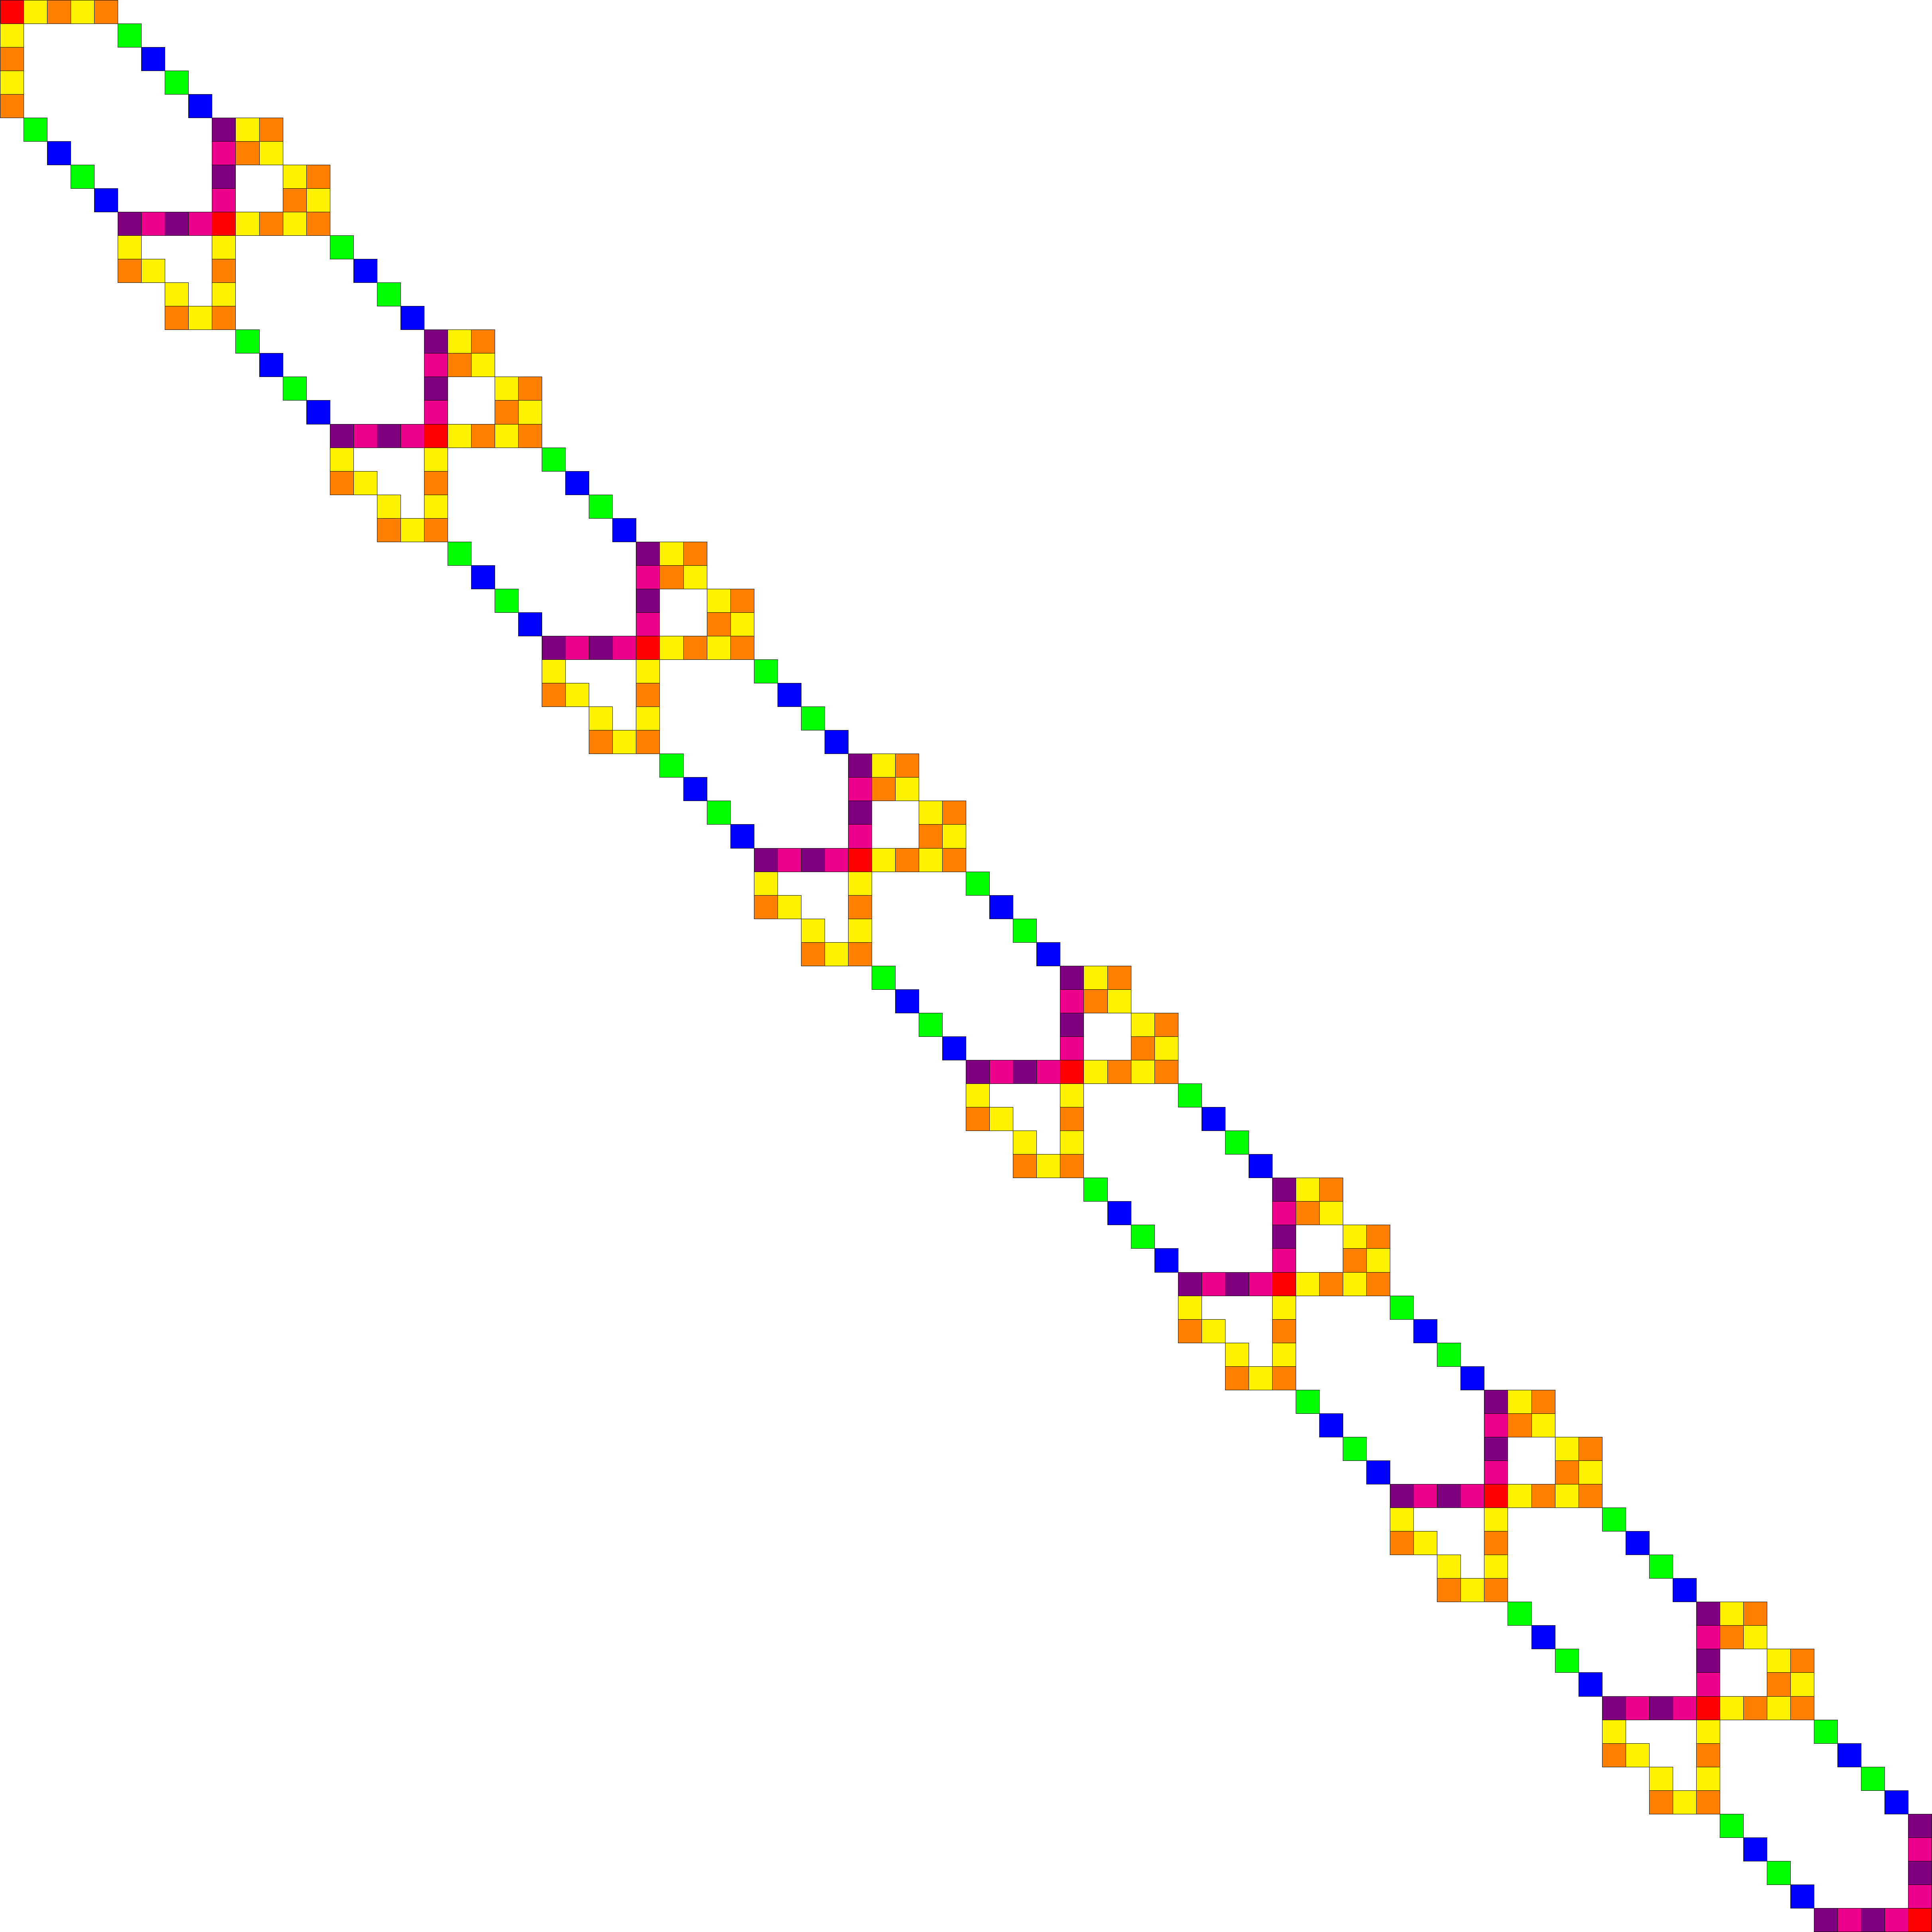
\includegraphics[scale=0.175]{figures/twoterm.pdf}
\hspace{0.2in}
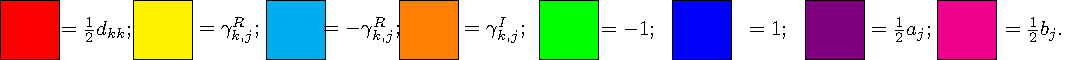
\includegraphics[scale=0.85]{figures/colorcode.pdf}
\end{center}
\caption{Pictorial description of the extended sparse matrix where $N=10$, $J_0=0$, and $J=2$, following
the example shown in \citet{Ambikasaran:2015}.}
\figurelabel{matrix_structure}
\end{figure}

{\bf Should I give some examples of this?  Some pseudocode?}

\bibliography{genrp}

\end{document}
